% !TeX program = xelatex
% 基于团队模板，源仓库提交 03fa14a910d15a2c8e45b0b1e20048ed6c135eaf；正文为待补骨架。
%=====================================================================
% 华为杯研究生数模竞赛 · 官方风格 LaTeX 模板（AI 产线用）
% 适配：附件2《论文格式规范》全部硬规 + 附件3官方Word模板实测参数
%   （2026-09-22 经 Word COM 读取附件3 + PDF 文本层逐项核对）
%   - 页边距：上3.0 / 下1.75 / 左2.25 / 右2.25 cm（=官方Word模板节参数）
%   - 摘要页骨架照附件3：赛事名三行（华文新魏18/22/22pt）
%     + "题 目：___"（隶书18pt标签，题目文字三号黑体——附件2规定）
%     + "摘 要：/关键词："（隶书18pt标签，内容小四宋体）
%   - 一级标题四号黑体居中；正文小四宋体；单倍行距
%   - 无页眉；页码页脚中部小五、阿拉伯数字自摘要页起连续（封面节官方自带"0"）
%   - 封面：官方Word模板填好后导出PDF（封面.pdf），本模板自动嵌入
% 编译：xelatex 论文模板_官方风格.tex  （需编译两遍使目录/引用稳定）
%=====================================================================
\documentclass[12pt, a4paper]{ctexart}
% ---- 字体：使用 Windows 系统中文字体（宋体/黑体/华文新魏/隶书），无需额外安装 ----
% ---- 字体：使用 Windows 系统中文字体（宋体/黑体/华文新魏/隶书），无需额外安装 ----
% 西文＝Times New Roman（等宽也用 Times：2025A 国一实测连 JSON 字段名都是 TimesNewRomanPSMT，
%   无 Courier；官方附件2 仅规定汉字宋体，西文按中文 Word 默认）。
\setmainfont{Times New Roman}
\setmonofont{Times New Roman}
\setCJKmainfont[AutoFakeBold=3.0, AutoFakeSlant=0.2]{SimSun}
% \textbf 中文粗体修复（2026-09-26）：\songti 切换的是 ctex 内部 zhsong 族，
% 绕过上面 mainfont 的粗体配置，导致正文 \textbf 静默回退常规字重（V008 起词条加粗未渲染）。
% 重定义 zhsong 族挂 AutoFakeBold，\songti 路径即渲染伪粗宋体（与 2025A 国一 Word 伪粗同视觉）。
\setCJKfamilyfont{zhsong}[AutoFakeBold=3.0]{SimSun}
\setCJKsansfont{SimHei}
\setCJKfamilyfont{xinwei}{STXinwei}   % 华文新魏：官方模板赛事名三行
\setCJKfamilyfont{lishu}{LiSu}        % 隶书：官方模板"题 目/摘 要/关键词"标签

\usepackage[a4paper, left=2.25cm, right=2.25cm, top=3.0cm, bottom=1.75cm, footskip=12pt]{geometry}
\usepackage{amsmath}
\usepackage{unicode-math}   % 数学整体 Times 化：newtxmath 在 xeCJK 下数学数字/重音/\mathrm 漏回 CMR，换 OpenType 方案
\setmathfont{TeX Gyre Termes Math}   % Times 的 OpenType 数学版，全部数学字符单一 Times 族
\usepackage{graphicx}
\usepackage{booktabs}          % 三线表
\usepackage{multirow}
\usepackage{caption}
\usepackage{pdfpages}          % 嵌官方封面用
\usepackage{fancyhdr}          % 页码字号对齐官方（9pt≈小五）
\usepackage[colorlinks, linkcolor=black, citecolor=black, urlcolor=black]{hyperref}

% ---- 页眉页脚：无页眉 + 页码页脚中部小五（官方模板页码为 9pt Times）----
\fancypagestyle{plain}{%
  \fancyhf{}%
  \fancyfoot[C]{\zihao{-5}\thepage}%
  \renewcommand{\headrulewidth}{0pt}}
\pagestyle{plain}

% ---- 标题层级格式：一级=四号黑体居中（附件2 规定）；二三级=小四宋体加粗（2025A 国一实测：
%   二级标题 SimSun 12pt 加粗、黑体仅一级使用；官方对二三级无规定，按主基准口径）----
\ctexset{
  section = {format = {\centering\heiti\zihao{4}}, beforeskip=12pt, afterskip=8pt},
  subsection = {format = {\raggedright\songti\bfseries\zihao{-4}}, beforeskip=8pt, afterskip=6pt},
  subsubsection = {format = {\raggedright\songti\bfseries\zihao{-4}}, beforeskip=6pt, afterskip=4pt}
}
% ---- 图表题注：小五宋体，图题下方/表题上方，编号按节 ----
\captionsetup{font={small}, labelsep=quad}
% ---- 行距：正文基线距 ≈ 19.9pt，对齐 2025A 国一实测主峰（Word"单倍行距"的实际获奖解读；
% 官方附件2 字面"单倍"≈15.6pt，无获奖论文实际采用；ctex 默认 1.3=18.7pt 偏紧）----
\linespread{1.38}
\emergencystretch=1.5em   % Times+伪粗变宽后的临界溢出兜底（允许断行器更大伸展，避免零星 Overfull）
\setcounter{tocdepth}{2}  % 目录到二级（对齐 2025A 国一目录粒度；三级全收会溢出两页）

% ---- 正文显式小四宋体（不依赖 12pt 隐式默认，换文档类不破）----
\AtBeginDocument{\zihao{-4}\songti}

% ---- 宽表降压宏：5列以上中文表头三线表用它包住 tabular 防超宽 ----
% 用法：\begin{table}[h]\centering\caption{...}\widetable{\begin{tabular}{...}...\end{tabular}}\end{table}
\newcommand{\widetable}[1]{{\small\setlength{\tabcolsep}{3.5pt}#1}}
% 长公式放不下时：拆式 + \notag 续行，或多行 aligned 环境；编译后 grep Overfull 必须为零

\usepackage{tabularx,xcolor,longtable}
\graphicspath{{figs/}}
\newcommand{\pending}[1]{\par\noindent\textcolor{red!65!black}{\textbf{[TODO / 待补]} #1}\par}
\begin{document}

% ===================== 封面（官方Word模板导出的PDF）=====================
% 赛期操作：用 Word/WPS 打开附件3官方模板 → 填队伍信息 → 导出 PDF 为"封面.pdf"
% → 与本文件同目录，取消下行注释即可嵌入。
% 页码联动（已核官方参数）：官方封面节页码从"0"起、导出PDF自带页脚"0"；
% 嵌入后下方 \setcounter{page}{1} 使摘要页从"1"起，与官方逻辑完全一致。
% \includepdf[pages=1, pagecommand={\thispagestyle{empty}}]{封面.pdf}

% ===================== 摘要页（页码从此页起为 1）=====================
% 骨架照官方附件3逐项复刻（COM+PDF文本层核对）：
%   赛事名三行 = 华文新魏 18/22/22pt；"题 目/摘 要/关键词"标签 = 隶书18pt。
% 附件2规定"论文题目用三号黑体"——指填入下划线内的题目文字本身。
% ⚠ 摘要预算：骨架头部约占版心 1/4（约10行当量），摘要正文须控制在版心 70% 以内，
%   否则关键词溢出到第2页形成"幽灵页"（2026-09-22 全链演练实测）。
\setcounter{page}{1}
\vspace*{0.3cm}   % 官方摘要页赛事名首行 y≈123pt（版心顶下约38pt，已含center环境间距）
\begin{center}
  {\CJKfamily{xinwei}\zihao{-2} 中国研究生创新实践系列大赛}\\[10pt]
  {\CJKfamily{xinwei}\zihao{2} “华为杯”第二十三届中国研究生}\\[10pt]
  {\CJKfamily{xinwei}\zihao{2} 数学建模竞赛}
\end{center}

\vspace{1.8em}
\begin{center}
  {\CJKfamily{lishu}\zihao{-2} 题\quad 目：}\underline{\makebox[8.6cm][c]{\heiti\zihao{3} 多核调度论文标题（待定）}}
\end{center}

\vspace{1.8em}
\noindent{\CJKfamily{lishu}\zihao{-2} 摘\quad 要：}\par
\vspace{2pt}
\zihao{-4}
\pending{摘要 TODO：研究背景与总体任务；分别概括问题一、问题二、问题三的建模思路、采用方法、核心结果与验证；给出总体结论与适用范围。正文模型与结果稳定后撰写，不提前填入方法名称或量化结论。}

\vspace{1.2em}
\noindent{\CJKfamily{lishu}\zihao{-2} 关键词：}{\zihao{-4} 待根据最终模型填写}

\newpage
% ===================== 目录页（页码按官方规则自摘要页连续编号；"目录"标题随一级标题样式=四号黑体居中）=====================
\tableofcontents

\newpage
% 冻结目录见 paper_outline.md；正文按章节拆分维护。
% 结构版本 v0.2：用户已确认审阅稿（D015）；以下均为写作说明。
% 第一章 1.1–1.5 已全部定稿（V003–V010，均经用户审定）；章节级待补标记已清零（V010）。
\section{问题综述}\label{sec:problem}

\subsection{问题背景}\label{sec:background}
% 状态：V003（2026-09-25 用户对话逐句审定，1.1 定稿；段一沿用 V002 方案 A 并挂文献 hennessy2019golden / jouppi2017tpu，Crossref 核验；段二至四按版本 C 结构重写，Makespan 撤出 1.1 首现移至 1.4，D021）。素材：S01 官方题面（导语、1.1--1.3、1.5、算法优化方向）改写；不含实验数据，不提及具体方法名。

随着深度神经网络模型规模与计算复杂度持续增长，人工智能推理任务对计算吞吐、执行时延与能效提出了更高要求。神经网络处理器（Neural Processing Unit，NPU）针对神经网络计算中矩阵与向量运算密集的特点进行专用化设计，相比通用处理器能够更高效地执行推理计算\cite{hennessy2019golden,jouppi2017tpu}；然而，受制造成本、功耗与散热等因素限制，单个 AI 核心的计算能力难以持续提升。为突破单核算力瓶颈，多核 NPU 通过多个 AI 核心协同执行计算任务，成为进一步提升并行能力与能效的主流架构。

典型的多核 NPU 由多个同构的 AI 核心构成：每个核心配置矩阵计算单元（Cube）、向量计算单元（Vector）、数据搬运单元以及私有 L1/UB 缓存；所有核心共享核外主存（DDR），对 DDR 的读写共同竞争固定的总物理带宽。神经网络计算本身可表示为一张有向无环图（Directed Acyclic Graph，DAG），称为计算图：操作节点表示一次计算或数据搬运，张量节点表示计算的输入、中间结果与输出，节点间的有向边表示数据依赖。由于实际神经网络计算涉及的数据规模通常远大于单核缓存容量，执行时还需将计算拆解为可在核内执行的细粒度操作及相应的张量数据块；本题给定的计算图即以这类细粒度操作、张量及其数据依赖关系为基本描述对象。

在多核 NPU 上高效执行计算图，需要联合确定三个相互耦合的决策：将完整计算图划分为若干子图，将子图分配到各核心，并确定每个核心上的子图执行顺序。这一问题的困难源于\textbf{并行性、数据局部性与通信开销之间的固有权衡}：细化切分能够增加可独立调度的子图数量，却可能削弱数据局部性，带来跨子图边界的数据搬运与对同一输入的重复读取；将依赖关系紧密的节点聚合于同一子图，有利于中间数据的核内驻留与复用，却可能减少可独立调度的子图数量，并因子图规模增大而加重核内缓存压力，在容量不足时引发缓存换入换出。此外，各核心的核外数据搬运共同竞争有限的 DDR 带宽，局部并行度较高的调度方案并不一定取得更短的总体执行时间。

因此，多核调度本质上是一个受数据依赖、核内缓存容量、计算流水线与共享带宽共同约束的联合优化问题。进一步地，核间同步机制与共享 L2 缓存的引入会改变子图间的数据通信与缓存复用方式，对调度方法在不同硬件场景与核心数量下的适应能力提出了更高要求。如何在上述约束与硬件条件下生成合法且高效的多核切图与调度方案，是多核 NPU 高效运行所需解决的核心问题。

\subsection{多核 NPU 系统与计算图分析}
% 状态：1.2 引语段 + 1.2.1 定稿（V004，用户逐句审定，A013）；1.2.2 定稿（V007，2026-09-25 用户逐句审定＋两轮 GPT 评审仲裁，A024）；1.2.3 定稿（V006，用户逐句审定，A021）。
为明确后续建模涉及的硬件约束、计算对象与调度方案表示，本节首先介绍多核 NPU 的硬件架构，随后说明计算图的结构与节点表示，并给出子图划分与任务调度的组织方式。

\subsubsection{多核 NPU 硬件架构}
% 状态：V004 定稿（2026-09-25 用户逐句审定）。素材：题面 1.1/1.2/1.5、附录 A、B.4、D.5；无实验数据、无方法名；不挂文献（"商用一致"断言过强已撤，Ascend 回 D024 候选池）。
题设多核 NPU 的核心执行资源包括四类执行管道：PIPE\_M 与 PIPE\_V 分别承载 Cube 矩阵计算与 Vector 向量计算；数据搬运管道 PIPE\_MTE2 负责 DDR$\rightarrow$L1/UB 与 UB$\rightarrow$L1 方向的搬运，PIPE\_MTE3 负责 L1/UB$\rightarrow$DDR 与 L1$\rightarrow$UB 方向的搬运。在官方评估模型中，同一管道上的操作串行执行，不同管道上满足数据依赖与资源约束的操作可并行执行，因此 Cube 与 Vector 可同时工作。

存储层级由核内私有缓存与核外共享主存构成：每个核心拥有私有 L1 缓存（524288 bytes，合 512 KiB）与 UB（131072 bytes，合 128 KiB），分别主要服务于 Cube 与 Vector 计算；所有核心共享的 DDR 提供固定的总物理带宽（60 bytes/cycle），由 DDR 服务的核外数据搬运共同竞争该带宽，而 L1 与 UB 之间的核内搬运只占用对应管道、不消耗 DDR 带宽。DDR 访问不按固定周期数结算，完成时间由搬运数据量与评估时刻的可用带宽共同决定。此外，问题三在上述结构基础上引入全核共享的只读 L2 缓存（容量 1 MB、读带宽 250 bytes/cycle，与 DDR 带宽相互独立），用于复用多核共享输入，其缓存机制与调度含义在第六章展开。多核 NPU 的固定硬件配置汇总于表~\ref{tab:hw-config}。

\begin{table}[htbp]
  \centering
  \caption{多核 NPU 固定硬件配置}
  \label{tab:hw-config}
  \widetable{\begin{tabular}{llp{5.9cm}}
    \toprule
    部件 & 参数 & 数值 \\
    \midrule
    L1 缓存（每核私有） & 容量 & 524288 bytes（512 KiB） \\
    UB（每核私有） & 容量 & 131072 bytes（128 KiB） \\
    DDR（全核共享） & 总物理带宽 & 60 bytes/cycle \\
    L2 只读缓存（全核共享，仅问题三） & 容量 / 读带宽 & 1048576 bytes（题面记为 1 MB）/ 250 bytes/cycle \\
    \bottomrule
  \end{tabular}}
  \begin{minipage}{0.9\linewidth}
    \small 注：1 KiB = 1024 bytes；取值来自题面附录 A 及 B.4 固定配置。
  \end{minipage}
\end{table}

% 图 F05（1.2.1 配图）：用户以 PowerPoint 手工绘制的终图 figs/F05_hw_abstraction.png（pptx 源文件待归档 figs/）；matplotlib 参考版与脚本见 figs/F05_hw_abstraction_scriptref.* 与 scripts/fig_F05_hw_abstraction.py（来源登记见 05/figure_registry、09、08/D034）。
\begin{figure}[htbp]
  \centering
  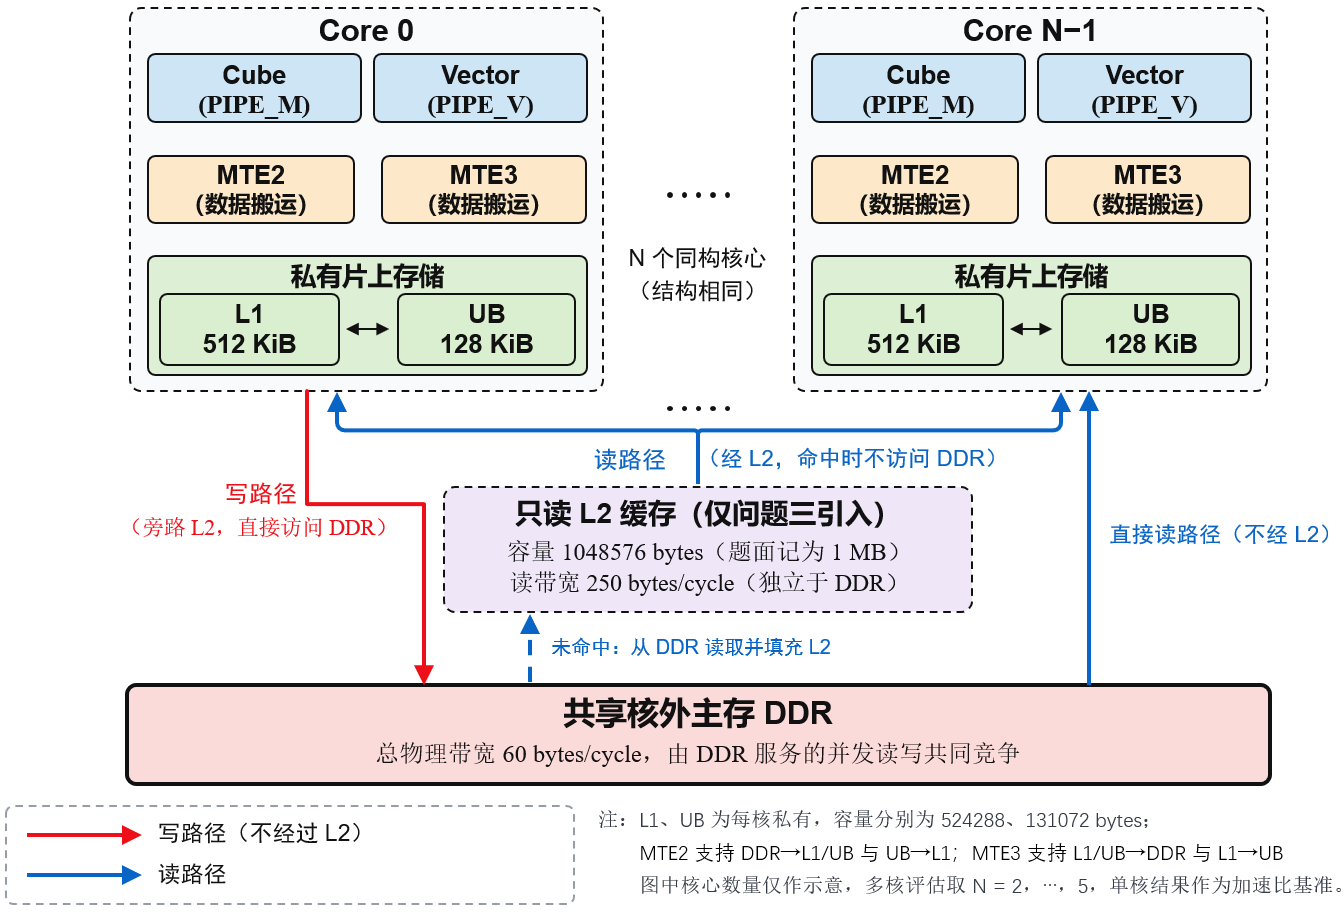
\includegraphics[width=0.92\textwidth]{F05_hw_abstraction.png}
  \caption{多核 NPU 硬件抽象与存储层级示意图}
  \label{fig:hw-arch}
\end{figure}

\subsubsection{计算图结构与节点表示}
% 状态：V007 定稿（2026-09-25 用户逐句审定＋两轮 GPT 评审仲裁，A024）。素材：题面 1.2、附录 B.3/B.7；无实验数据、无方法名、不挂文献。X01：正文按题设文字口径并加"按照题设给定的计算图格式"限定（官方 stub 代码 _build_op_adjacency 允许 Op→Op 直连边，T014 核验后如证实全量输入满足可去限定）；s_t 的跨边界搬运语义归 1.2.3 评估器句。1.2.3 字段名同轮统一 \texttt（纯排版，D031 不占号）。
% 图位（F20 输入计算图最小示例；草图 v3.1 已交待审核，tex 插图随 F06/F20 插图轮进行，登记见 registry/05）：以题面附录 B.7 最小例（DDR Tensor→COPY_IN→UB Tensor→ADD→UB Tensor→COPY_OUT→DDR Tensor）展示两类节点、边方向与 pos 属性；图管关系、表管字段，节点只标代表性属性（Tensor: pos/size，Op: op/pipe/cycles），不复刻题面图 1 矩阵乘法例。
如 1.1 节所述，本题给定的计算图以细粒度操作、张量及其数据依赖关系为基本描述对象，整体构成有向无环图。形式上，将计算图记为 $G=(V,E)$：张量节点集合 $T$ 与操作节点集合 $O$ 不相交，共同构成节点集合 $V=T\cup O$，每个节点具有在同一计算图内全局唯一的整数 \texttt{id}。按照题设给定的计算图格式，有向边集合 $E$ 只允许张量节点与操作节点相连：对 $t\in T$、$o\in O$，边 $t\rightarrow o$ 表示张量 $t$ 是操作 $o$ 的输入，边 $o\rightarrow t$ 表示 $t$ 是 $o$ 的输出。由此，计算图具有张量与操作相连的二部结构（Tensor--Op 二部图），操作之间的数据依赖经由其间的张量传递；边本身不设置独立的数据量字段，相关数据规模由关联张量的 \texttt{size} 属性给出。

张量节点（Tensor）表示一块数据，记作 $t\in T$，可作为计算图的输入、输出或中间结果，包含位置与数据大小两类属性。位置属性 \texttt{pos} 表示输入图规定的逻辑存储位置，可取 DDR、L1 或 UB：计算图的输入、输出张量位于 DDR，中间张量位于核内缓存（L1 或 UB）。数据大小 $s_t$（字段 \texttt{size}）为张量占用的字节数，取非负整数，同时用于核内容量检查与数据搬运量计算。

操作节点（Op）表示一次计算或数据搬运，记作 $o\in O$，包含操作类型、执行管道与周期字段三类属性。操作类型 \texttt{op} 标识具体操作：COPY\_IN 将数据从 DDR 搬入核内缓存，COPY\_OUT 将数据从核内缓存搬回 DDR，ADD、MUL 等为在指定计算单元上执行的核内计算操作。执行管道 \texttt{pipe} 指定操作占用的硬件流水线，取 1.2.1 节所述四类执行管道之一：核内计算操作在 PIPE\_M 或 PIPE\_V 上执行，搬运操作占用相应的数据搬运管道。对核内计算操作，字段 \texttt{cycles} 给出其执行周期数 $c_o$，由计算图直接给定；对于访问 DDR 的搬运操作，其最终耗时不由 \texttt{cycles} 直接确定，而由搬运数据量与评估时刻的可用带宽共同决定（见 1.2.1）。

输入计算图采用 JSON 格式，顶层包含 \texttt{tensors}、\texttt{ops} 与 \texttt{edges} 三个数组，分别记录张量节点、操作节点与有向边，各字段含义汇总于表~\ref{tab:input-format}。题设对输入计算图进一步保证：每个 DDR 输入只搬入一次、每个最终结果只搬出一次；中间计算不与 DDR 交换数据；单个计算操作的输入、输出总量不超过相应核内缓存容量。

\begin{table}[htbp]
  \centering
  \caption{输入计算图 JSON 字段说明}
  \label{tab:input-format}
  \widetable{\begin{tabular}{llp{5.9cm}}
    \toprule
    数组 & 字段 & 含义与取值 \\
    \midrule
    \texttt{tensors} & \texttt{id} & 张量节点 id，与其他节点共享全局唯一编号 \\
     & \texttt{pos} & 逻辑存储位置：DDR / L1 / UB \\
     & \texttt{size} & 张量大小 $s_t$（bytes，非负整数） \\
    \texttt{ops} & \texttt{id} & 操作节点 id，与其他节点共享全局唯一编号 \\
     & \texttt{op} & 操作类型：COPY\_IN / COPY\_OUT / ADD / MUL 等 \\
     & \texttt{pipe} & 执行管道：PIPE\_M / PIPE\_V / PIPE\_MTE2 / PIPE\_MTE3 \\
     & \texttt{cycles} & 周期字段；核内计算操作据此确定执行周期 $c_o$ \\
    \texttt{edges} & \texttt{source} / \texttt{target} & 边两端节点 id；题设规定为 Tensor\,$\rightarrow$\,Op 或 Op\,$\rightarrow$\,Tensor \\
    \bottomrule
  \end{tabular}}
  \begin{minipage}{0.9\linewidth}
    \small 注：字段与约束来自题面附录 B.3；数值字段均为非负整数，所有节点 \texttt{id} 在同一计算图内全局唯一。
  \end{minipage}
\end{table}

\subsubsection{子图划分与任务调度描述}
% 状态：V006 定稿（2026-09-25 用户逐句审定，A021）。素材：题面 1.2/1.3/1.5、附录 B.5/B.7/D.1/D.2；无实验数据、无方法名、不挂文献。延后项（V009 轮更新去向）：延迟常量（100/1000/500 cycles）不入 1.5，留第四至六章对应模型与实验设置；$C_{\mathrm{inner}}/C_{\mathrm{cross}}$ 仅在后文确有使用时引入；Makespan 等指标名不提前出现（D021 首现 1.4）；场景 B 驻留代价与容量影响按拆层落实——问题定义层在 1.5.2（V009），驻留机理与权衡分析留第五章（跨节去重）。COPY\_IN/COPY\_OUT 为 1.2.2 待定义节点类型，1.2.2 落稿时衔接。
在计算图表示的基础上，多核调度按两个相互衔接的过程展开：切图通过确定核内操作节点的子图归属，将完整计算图划分为若干子图，子图数量不作限制；子图调度将各子图分配到具体核心，并确定每个核心上的子图执行顺序。划分得到的每个子图以子图 id（Subgraph id，下文简称 sgid）标识。切图方案以映射表 \texttt{node\_to\_subgraph} 表示：核内操作节点（即除 COPY\_IN 与 COPY\_OUT 两类数据搬运节点外的操作节点）各自映射到一个非负整数 sgid，且映射必须覆盖全部核内操作节点。跨子图的依赖边在子图层面构成子图依赖图；子图依赖图必须为有向无环图，即至少存在一个合法的拓扑序，否则切图方案无效。

子图在核心上的执行以任务（Task）为单位组织：Task 是 CPU 主控向单个核心一次下发并统一调度的最小执行单元，一个 Task 可包含一个或多个子图，对应关系由硬件场景决定。场景 A 无核间同步机制，每个子图独立构成一个 Task；Task 之间不保留核内缓存状态，跨子图数据都必须经 DDR 中转。场景 B 引入核间同步机制：在官方评估规则下，同一核心上的全部子图合并为一个 Task，前序子图的输出可驻留在 L1/UB 中供后续子图直接使用，Task 内的子图边界不再插入数据搬运；跨核依赖则由源核心将数据写入 DDR 并发送同步信号，目标核心收到信号后读取。问题三沿用场景 B 的 Task 组织方式，仅增加全核共享的只读 L2 缓存（见 1.2.1）。

子图调度方案以 \texttt{core\_schedules} 表示：由 $N$ 个 sgid 列表组成（$N$ 为核心数量），外层下标对应核心编号，内层列表按执行顺序依次给出该核心分得的 sgid，允许为空，即允许个别核心不分得任何子图；全部列表合并后，每个 sgid 必须且只能出现一次（即每个子图恰好被调度一次），同一核心内的执行顺序还不得违反子图间依赖，否则子图调度方案无效。方案本身只给出子图层面的归属、分核与顺序；官方评估程序根据原始计算图、切图方案、子图调度方案及对应场景规则，重建跨 Task 边界的数据搬运，再确定各 Task 内部的核内操作顺序，并在共享带宽约束下模拟多核并行执行，最终输出各项评估指标。

\subsection{输入图解析与调度特征提取}
% 状态：V010 定稿（2026-09-26 用户逐段审定＋三轮 GPT 评审仲裁，AI-09/A046）。素材：官方评估器与 stub 代码核验（校验/调度两条建图视图、合法性两层、P3 缓存键=COPY_IN 输出张量 logical\_tid 跨核共享）、v5 两段式实现核料（实际特征清单＋"未找到"清单：无独立输入校验/无静态容量约束/接受准则只看 Makespan）、2025A 国一 1.2/1.3 写法对照（解析入一章、特征公式后移）；无实验数据、无方法名、不挂文献。要点：三层信息框架（直接读取／静态推导／评估获得或统计）贯穿全节；COPY 收缩细节与"与官方评估程序一致"整称断言撤出（求解侧辅助索引＋官方为准）；L2 复用对象不限定 DDR 图输入（同一张量跨核重复 COPY\_IN 共享缓存键）；负载项章节指向用"后续"（三问共用）。1.3 无图表（D045 复核）。延后项：分管道计算量等特征的正式符号留第四至六章首用处定义（D039 符号三处分工）；术语候选（多消费者张量/分管道计算量）待第四章与 2.1 使用时对齐入 06（Needs-integration）。
1.2 节说明了计算图与调度方案的表示。在此基础上，本文求解流程对输入计算图完成解析与信息提取：先由输入文件构建图结构与依赖关系（1.3.1 节），再从中得到支撑切图与调度构造、评价的各类信息（1.3.2、1.3.3 节）。按照获取方式，这些信息分为三层——直接读取的输入字段属性、由图结构与候选方案静态推导的特征、只能由评估过程获得或基于评估结果统计的指标。

\subsubsection{图结构解析}
求解流程读入 1.2.2 节所述 JSON 格式的输入计算图，为张量节点与操作节点分别建立属性表，并由边表建立张量与操作之间的生产、消费关联：指向操作节点的边将其记为该操作的输入张量，由操作节点引出的边将其记为该操作的输出张量。在张量—操作关联的基础上，为参与切图的核内操作节点（见 1.2.3 节）建立前驱与后继依赖索引，作为后续结构分析与候选方案构造的处理基础。该索引是求解侧的辅助表示，不改变输入计算图本身；方案的合法性判定与正式执行过程始终以官方评估程序为准。

依托该依赖索引可获得核内操作层面满足数据依赖约束的拓扑次序；输入计算图本身的无环性由官方评估入口统一校验。输入图与候选方案的合法性均由对应官方评估入口统一检查：基础校验涵盖输入字段类型与取值、节点编号全局唯一、边端点合法以及 1.2.3 节所列的方案条件，场景相关的执行可行性由对应问题的评估流程继续检查；求解流程不另设与官方并行的判定口径。候选切图方案产生后，将核内操作间的依赖按 \texttt{node\_to\_subgraph} 映射聚合：两端分属不同子图的依赖收缩为对应子图间的依赖边，由此构建子图依赖图，并以拓扑排序检验其无环性。

\subsubsection{计算与通信特征提取}
第一层信息由输入字段直接读取。1.2.2 节表~\ref{tab:input-format} 所列属性在调度中各司其职：字段 \texttt{cycles} 给出的执行周期 $c_o$ 度量核内计算操作的开销，是各类计算量统计的基本单元；字段 \texttt{size} 给出的张量大小 $s_t$ 以字节计量数据规模，是搬运量与存储占用的基本依据；执行管道 \texttt{pipe} 区分操作占用的资源维度，使负载可按管道分别核算；位置属性 \texttt{pos} 区分核内与核外数据；操作类型区分参与划分的核内操作与承担边界搬运的两类 COPY 操作。字段含义不再复述，以下只说明在其之上构造的调度特征。

第二层特征由图结构与候选分组静态推导，不经评估即可算得，对任意给定的操作分组均可计算，候选切图方案下即取各子图。分管道计算量将组内操作按执行管道分别累计执行周期（单位 cycles）；由于 Cube 与 Vector 两类计算管道可并行执行（1.2.1 节），计算负载须分管道核算而非合并为单一总量，该特征构成后续各核心负载估计的基础。跨组生产—消费张量字节把生产方与消费方分属不同分组的张量，按其大小累加到分组对上（单位 bytes），刻画候选划分形成的潜在边界数据规模；当核心分配形成跨 Task 或跨核边界时，该量可用于估计 DDR 通信需求，场景 B 下同核的生产—消费对可经核内驻留复用避免搬运（1.2.3 节），实际额外搬运量仍以官方评估结果为准。多消费者张量记录被两个及以上分组消费的张量的大小与消费方集合，为跨组通信与潜在重复读取分析提供结构信息，其与共享 L2 缓存复用的关联见 1.3.3 节。

\subsubsection{缓存相关特征提取}
与核内存储相关的信息来自张量属性与依赖结构。位置属性把张量分为核内驻留（L1 或 UB）与核外（DDR）两类，张量大小给出占用字节数；由生产—消费关系可确定各张量的产生端、消费端与复用关系，为判断潜在驻留范围与缓存压力提供结构信息。题设已保证单个操作的输入输出总量不超过相应核内缓存容量（1.2.2 节）。对子图或 Task 整体的实际驻留峰值与缓存换入换出（spill），本文不作静态近似：二者由官方评估程序的核内调度在评估中确定。因此，本文不把分组内张量大小之和当作容量约束使用；容量相关影响经由评估结果体现——spill 产生的搬运计入总额外数据搬运量，并通过对总体执行时间的作用进入候选方案的评估比较。

与共享 L2 缓存相关的静态访问特征是同一张量跨核重复读取的识别：当核心分配使多个核心对同一张量各自发起 COPY\_IN 访问时，该张量成为潜在的复用对象，其字节量与消费方分布（即 1.3.2 节的多消费者张量信息）刻画可复用空间；其与切图、分配及执行顺序的关联见 1.5.3 节，缓存机制与利用分析见第六章，Cache 命中率与命中字节由评估过程反馈获得。综上，本文调度的信息基础分为三层：直接读取的输入字段属性（1.2.2 节）、由图结构与候选方案静态推导的特征（1.3.2 节与本节），以及评估获得或基于评估结果进一步统计的性能指标——总体任务执行时间、总额外数据搬运量、Cache 命中率及加速比（1.4 节）。前两层支撑候选方案的构造与静态代价刻画，第三层用于方案评价与结果统计；其中总体任务执行时间作为候选筛选与方案改进的直接评价依据，其余指标用于辅助分析和结果报告。各类信息在第四至六章中的具体使用方式随相应模型与算法展开。

\subsection{名词解释}
% 状态：V008 定稿（2026-09-25 用户逐句审定＋四轮 GPT 评审仲裁，A029）。素材：题面 1.4 评估指标整节、问题一加速比定义与脚注 [^2][^3]、1.2 各定稿节；遵循 D036 词条自足原则（定义可复述、机制不重复）。符号首现：S_{k,i}、T_{1,i}、T_{k,i}、\bar S_k、m，3.2 符号表（TBL-003）届时收录；单核基准构造（启发式整图核内调度固定结果）与 P3 相对加速比定义留实验章/第六章；Makespan 与总额外数据搬运量首现本节（D021）。
本节对后文频繁使用的主要术语与评价指标作统一说明；相关硬件结构、计算图表示与调度方案的机制细节见 1.2 节，各评价指标在第四至六章的实验中按本节口径统计与报告。

\begin{itemize}
\item \textbf{NPU（神经网络处理器）}：面向神经网络计算中矩阵与向量运算密集的特点进行专用化设计的处理器；本题平台由 $N$ 个同构 AI 核心构成多核 NPU，正文中的“核心”均指 AI 核心。
\item \textbf{计算图（DAG）}：描述神经网络计算的有向无环图，操作节点与张量节点经有向边连接，边方向表达数据依赖。切图与子图调度均以计算图为直接对象。
\item \textbf{Tensor（张量节点）}：计算图中承载数据的节点，可表示输入、输出或中间结果。张量的数据大小是核内容量检查与数据搬运量计算的基本依据。
\item \textbf{Op（操作节点）}：计算图中表示一次计算或数据搬运的节点。核内计算操作（如 ADD、MUL）在相应计算单元上执行，COPY\_IN 与 COPY\_OUT 两类搬运操作负责核内缓存与 DDR 之间的数据交换。
\item \textbf{Pipe（执行管道）}：操作执行时占用的硬件流水线，本题包括 PIPE\_M、PIPE\_V、PIPE\_MTE2 与 PIPE\_MTE3 四类。在官方评估模型中，同一管道上的操作串行执行，不同管道上的操作在满足依赖与资源约束时可并行。
\item \textbf{Subgraph（子图）}：切图得到的核内操作节点分组，是核心分配与执行顺序的基本单位，子图数量不作限制。COPY\_IN 与 COPY\_OUT 两类搬运节点不参与子图分配。
\item \textbf{sgid（子图 id）}：子图的标识，取非负整数。切图方案以核内操作节点到 sgid 的映射表达，子图调度方案以各核心上的 sgid 有序列表表达。
\item \textbf{Task（任务）}：CPU 主控向单个核心一次下发并统一调度的最小执行单元，可包含一个或多个子图：场景 A 中每个子图独立构成一个 Task，场景 B 中同一核心上的全部子图合并为一个 Task。Task 的组织方式影响跨子图数据能否在核内驻留复用以及是否需要经 DDR 搬运。
\item \textbf{缓存换入换出（spill）}：官方评估程序在核内调度阶段因 L1/UB 容量不足自动插入的搬运：换出将驻留数据写回 DDR，换入在其再次使用前搬回。二者消耗 DDR 带宽并计入额外数据搬运量。
\end{itemize}

在上述术语的基础上，本文采用以下指标评价多核切图与调度方案的性能。

\begin{itemize}
\item \textbf{总体任务执行时间（Makespan）}：最重要的评估指标，指官方评估程序完成多核模拟后，所有操作结束时刻的最大值，单位为时钟周期。
\item \textbf{总额外数据搬运量}：次要指标，指相对于原始计算图已有 DDR 搬运、由切图与调度额外产生的 DDR 搬运字节数；新增搬运主要来自跨 Task 边界数据、对同一输入的重复读取与缓存换入换出。
\item \textbf{加速比}：对测试用例 $i$ 的 $k$ 核配置，定义
  \[ S_{k,i}=\frac{T_{1,i}}{T_{k,i}} \]
  其中 $T_{1,i}$ 与 $T_{k,i}$ 分别为该用例的单核基准 Makespan 与 $k$ 核多核评估所得 Makespan，单核加速比定义为 1。对包含 $m$ 个测试用例的测试集，平均加速比定义为
  \[ \bar{S}_k=\frac{1}{m}\sum_{i=1}^{m} S_{k,i} \]
  即取各测试用例加速比的算术平均，而非单核总时间与多核总时间之比。问题三另使用相对无 L2 基线的加速比，见第六章。
\item \textbf{Cache 命中率（仅问题三）}：次要指标，指可由只读 Cache 服务的 COPY\_IN 访问中，命中字节数占总访问字节数的比例，用于观察只读 Cache 对多核共享输入访问的覆盖程度。
\end{itemize}

\subsection{拟解决的问题}\label{sec:problems}
% 状态：V009 定稿（2026-09-26 用户对话审定＋四轮 GPT 评审仲裁，A036）。写法对照 2025A 国一 1.5：取其职责单一纪律（只答"解什么、题面要什么结果"），按冻结大纲改为总起段＋TBL-001＋三个单段小节；"为什么难"归第二章、驻留机理归第五章、结果展示集中表内（07 窗口表 W-A"每问三段式"提示被本定稿取代，用户确认）。素材：题面 1.3、1.5 硬件场景、问题一～三题述与脚注 1、附录 B.6/D.2；无实验数据、无方法名、不挂文献。
在 1.2 节的计算图与调度方案表示、1.4 节的评价指标基础上，本题要求提出高效且效果良好的多核切图与调度方法：对给定计算图与核心数量，联合确定各核内操作节点的子图归属、子图的核心分配以及各核心上的子图执行顺序，在合理时间内生成合法的切图方案与子图调度方案，以\textbf{缩短总体任务执行时间}为主要目标并控制额外数据搬运。三个问题在方案层面直接输出的决策对象相同，差异主要来自硬件场景及对应的评估机制：问题一考虑无核间同步机制的场景 A；问题二引入核间同步机制，即场景 B，Task 组织方式与核内数据复用方式随之改变；问题三在场景 B 基础上引入全核共享的只读 L2 缓存。三问均要求算法适应核数变化、稳定而高效地生成高质量结果，其中问题一、二明确要求覆盖 2～5 核（“高效”指避免暴力迭代搜索，以单个用例在 5～10 分钟内给出结果为佳）。实验均在题目给定的全部测试用例和固定配置参数下完成；三问的硬件场景、核心任务与题面结果要求汇总于表~\ref{tab:problem-reqs}。

% 表 TBL-001（三问场景与交付对照表）：V009 首次成表，四列定版（问题/硬件场景/核心任务/题面结果要求，05 与 registry 已同轮同步列定义，D029）；交付说明只在本表出现，三个小节不再复述。与 2.5 TBL-002 分工（D042 编号顺延）：本表管题面任务与结果要求，机制差异与决策边界归 TBL-002（05 §"TBL-002 不并入 TBL-001"）。
\begin{table}[htbp]
  \centering
  \caption{三个问题的硬件场景、核心任务与题面结果要求}
  \label{tab:problem-reqs}
  \widetable{\begin{tabular}{lp{3.4cm}p{3.4cm}p{3.9cm}}
    \toprule
    问题 & 硬件场景 & 核心任务 & 题面结果要求 \\
    \midrule
    问题一 & 场景 A：无核间同步，每个子图独立构成一个 Task，跨子图数据均经 DDR 中转 & 建立场景 A 下的多核切图与调度模型，以缩短总体任务执行时间为主、兼顾总额外数据搬运量 & 正文：1～5 核平均加速比折线图；附录：逐用例 Makespan 与总额外数据搬运量；附件：可复现 Python 程序脚本 \\
    问题二 & 场景 B：引入核间同步，同核全部子图合并为一个 Task，同 Task 内直接复用核内驻留数据，跨核经 DDR 中转与同步信号 & 在问题一基础上，在严格满足 L1/UB 容量约束的前提下进一步缩短总体任务执行时间并减少额外数据搬运 & 与问题一相同（场景 B 下） \\
    问题三 & 在场景 B 基础上增加全核共享只读 L2 缓存（复用多核共享输入），Task 组织与问题二相同 & 在题目给定配置下，研究引入共享只读 L2 对多核切图与调度的影响，并建立相应模型 & 正文：无 L2 与只读 Cache 两种配置的 1～5 核对比曲线及相对无 L2 基线的加速比；附录：两配置逐用例 Makespan、总额外数据搬运量与 Cache 命中率 \\
    \bottomrule
  \end{tabular}}
  \begin{minipage}{0.9\linewidth}
    \small 注：三问在方案层面直接输出的决策对象相同，均为切图方案与子图调度方案（见 1.2.3 节）；本表依据题面问题一至三的要求整理。
  \end{minipage}
\end{table}

\subsubsection{问题一：场景 A 下的多核切图与调度}
% 状态：V009 定稿（同上）。要点：场景 A 事实层——每子图一 Task、跨子图必经 DDR 且不因是否同核而改变（附录 D.2）；不写"任意两子图单位通信成本相同"，避免与 Task 激活等待 100/1000 cycles 的不对称产生表面冲突；约束并列删除（合法性由"1.2.3 节全部合法性条件"承担，流水线/带宽属评估机制）；效率与实验要求只在总起段出现一次；交付只在表内。
如 1.2.3 节所述，场景 A 无核间同步机制：每个子图独立构成一个 Task，Task 间不保留核内缓存状态，跨子图数据均需经 DDR 中转，不因两个子图是否分配在同一核心而改变。问题一要求在此场景下建立多核切图与调度模型并设计求解算法：给定输入计算图与核心数量 $N$，为每个核内操作节点确定子图归属，并确定各子图的核心分配与各核心上的执行顺序，输出满足 1.2.3 节全部合法性条件的切图方案与子图调度方案，以缩短总体任务执行时间为主要目标，兼顾总额外数据搬运量。

\subsubsection{问题二：场景 B 下的多核切图与调度}
% 状态：V009 定稿（同上）。要点：方案表示与基本合法性条件沿用问题一；场景 B 三事实（合并 Task 带"在官方评估规则下"限定／同 Task 内复用／跨核 DDR＋同步信号）；驻留代价拆层——本节只保留问题定义层"复用避免边界搬运但驻留占用有限 L1/UB 空间"（引出严格容量约束），机理链（压缩中间子图空间、降低执行效率）与权衡分析留第五章，第二章是否先概括待其起草定（1.2.3 注记"留 1.5 问题二/第五章"在拆层下仍为真）；交付只在表内。
问题二将硬件场景由场景 A 换为场景 B，方案表示与基本合法性条件沿用问题一。场景 B 引入核间同步机制：如 1.2.3 节所述，同一核心上的全部子图在官方评估规则下合并为一个 Task，同 Task 内的子图可直接复用核内驻留数据，跨核依赖仍经 DDR 中转与同步信号传递。同核复用能够避免同 Task 内子图边界的数据搬运，但驻留数据持续占用有限的 L1/UB 空间；问题二因而要求在问题一的基础上建立适用于场景 B 的切图与调度模型，在\textbf{严格满足 L1/UB 容量约束}的前提下，进一步缩短总体任务执行时间并减少额外数据搬运。

\subsubsection{问题三：共享 L2 Cache 下的多核切图与调度}
% 状态：V009 定稿（同上）。要点：因果方向取题面原语——研究共享只读 L2 对多核切图与调度的影响（不加"性能"）；调度→访问模式→Cache 复用效果→时间为机理句而非任务定义；"题目给定的容量与带宽配置"限定（不解读为参数扫描）；两配置对照是任务组织方式留在正文，字段清单归表；P3 结尾不宣布额外搬运为优化目标（题面只要求报告）；补"设计求解算法"与 P1/P2 对仗。
问题三在场景 B 的基础上引入全核共享的只读 L2 缓存（见 1.2.1），用于复用多核共享输入，Task 组织方式与问题二相同，决策对象与合法性条件不变。该问题要求在题目给定的只读 L2 容量与带宽配置下，\textbf{研究共享只读 L2 对多核切图与调度的影响}，并建立相应模型、设计求解算法；切图、核心分配与执行顺序会改变共享输入的访问模式，进而影响 Cache 复用效果及总体执行时间。其任务以无 L2 与只读 Cache 两种配置的对照形式组织，用以比较共享只读 L2 对总体任务执行时间、总额外数据搬运量及 Cache 复用效果的影响。

% 结构版本：D042 五节结构（2.1 测试用例结构分析＋2.2–2.5）。本轮 V011 定稿（2026-09-26 用户对话审定＋三轮 GPT 评审仲裁，AI-12/A048，W-B 窗口）。
% 过程与裁决要点：核料＝三只读子代理（2025A 国一第 2 章写法／题面机制原句逐字摘录／D038 方法侧素材证据状态核验）；
% ①2.5 两段式总路线按 D038 粒度收窄——不出现 REINFORCE/采样解码/精修邻域/"解码代价项"，算法名归 4.4/4.5，场景差异表述升为"场景适配与评价环境"（用户确认；大纲 2.5 素材行字面含"离线 REINFORCE 训练／在线采样解码"，粒度注记待整合窗同步）；
% ②2.4 首句括注"L2 带宽与 DDR 带宽相互独立"保留（GPT 删除建议仲裁驳回、用户改判确认保留：1.2.1 已定稿该事实、1.5.3 有"容量与带宽配置"复述先例、后文"减轻 DDR 压力"需此机制支点；按 D048"信息主要载体＋再引用承担新作用"属合规回指；6.1 仍为 L2 机制唯一展开处）；
% ③"并行度上限"改称"结构并行潜力"（max(W_M,W_V)/CP 无严格上界推导，与 01_context §5.3/§5.4 上限措辞警示一致；T026 后若补推导可改回；大纲 2.1 字样待同步）；
% ④2.2 决策耦合句按场景 A 语境重分配（spill 归 Task 内容与容量、执行顺序管 Task 激活与等待；题面 1.3"同一核内的子图调度顺序影响依赖等待、张量驻留时间和缓存换入换出"句的驻留/换入换出含义主要落场景 B——5.1 起草时对齐口径，勿两章打架）；
% ⑤与 V010（1.3）跨窗对齐：2.1 建图注明求解侧辅助视图（1.3.1"官方为准"原则）；"多消费者张量""分管道计算量"沿用 1.3.2 术语；2.4 重复读取主语由"同一输入/Task"改"同一张量/核心"（1.3.3：L2 复用对象＝同一张量跨核重复 COPY_IN，不限 DDR 图输入）；
% ⑥2.1 数值冻结（D042 数值纪律，% TODO(T026) 源码注释不渲染；T026 出数后从"统计了什么"改写为"数据表明什么"，仅留 2～3 条支撑 4.3 的结论）；TBL-002 未写（仲裁"先无表起草"，定稿按篇幅定去留）；F01 引用句与 figure 环境随图定版补入。
% 素材：题面 1.1/1.2/1.3/1.4/1.5、问题一至三题述、附录 A/C.2/D；无实验数据、无方法名、不挂文献；写法对照 2025A 国一第 2 章（薄分析章：总起定性＋逐问一段＋技术路线图）。
\section{问题分析}\label{sec:analysis}

三个问题共享\textbf{统一的决策骨架}：直接可控的决策同为切图方案与子图调度方案（见 1.2.3 节），方案表示与基本合法性条件一致；差异不在决策对象，而在硬件场景及与之绑定的评价语义——问题二引入核间同步机制，问题三进一步引入全核共享的只读 L2 缓存，评价环境逐问扩展。求解困难的共同来源在于切图、核心分配与执行顺序三层决策的相互耦合：决策空间随操作节点数量与核心数量组合增长，而题设要求在可接受时间内稳定生成高质量方案、避免暴力迭代式搜索。本章 2.1 节先分析测试用例的结构特征，2.2～2.4 节分别讨论三个问题的核心权衡与求解困难，2.5 节在此基础上给出总体建模思路。

\subsection{测试用例结构分析}\label{sec:case-analysis}
% 状态：框架文字落稿（V011），数值冻结待 T026；判定口径随 TBL-012/F22 给出（图或表二选一，选型待真数据，registry F22 状态行待整合窗修正为"工具＋自测就绪、正式数据待 T026"）。
问题分析的对象除机制与约束外，还包括题目给定的测试用例本身：用例的规模、并行潜力与数据共享模式，决定了调度决策空间的基本形态。为刻画与切图决策相关的图结构，本节构建操作级依赖图：收缩张量中转节点，COPY\_IN 与 COPY\_OUT 节点按统计口径处理，建图规则随统计口径统一说明（求解侧辅助视图，正式执行以官方评估程序为准，见 1.3.1 节）。在此图上统计三类信息：一是规模与负载分布，包括操作数、张量数、边数、双管道负载比（由 1.3.2 节分管道计算量核算），并以双管道负载较大者与关键路长度之比刻画结构并行潜力；二是结构类型分布，将用例归入弱连通分量型、汇聚规约型、深链型与其他四类；三是共享数据特征，即多消费者张量（见 1.3.2 节）的数量与规模（对照 L2 容量）。
% TODO(T026, 数值冻结)：官方算例复算并登记 02 后补写——四类结构占比与代表用例、规模与结构并行潜力分布、多消费者张量规模与 L2 容量对照；引出"瓶颈落在可控决策空间"的判断（2.5 与 4.3 的动机链）。外部帖比例与审题报告旧数字（未复算）不入文。

\subsection{问题一分析}
场景 A 无核间同步机制，每个子图独立构成一个 Task，跨子图数据一律经 DDR 中转（见 1.2.3 节）。问题一的困难首先来自三个决策的耦合：切图决定子图粒度、跨子图通信边界以及单个 Task 的缓存工作集，核心分配决定负载分布与哪些数据依赖转为跨核等待，执行顺序则影响 Task 的激活与依赖等待时序；三者共同决定最终的并行收益与搬运代价，题设据此强调不能孤立优化任一环节。核心权衡在于\textbf{并行收益与搬运代价的对抗}：细化切分增加潜在可独立调度的单元，但可能带来更多边界搬运与对同一输入的重复读取；聚合可消除被合并边界上的搬运，却因子图规模增大而加重核内缓存压力，容量不足时评估程序自动插入缓存换入换出。场景 A 中，边界搬运与缓存换入换出同样由 DDR 服务、共同竞争固定的总带宽：提高并行度可能伴随更多并发搬运，从而加剧带宽争用、侵蚀并行收益；粒度变化同时改变两类搬运的规模与并发时序，并进一步影响可并行空间与负载均衡。在满足 1.2.3 节全部合法性条件的前提下，于组合增长的决策空间中高效构造并持续改进方案，构成问题一在求解层面的首要困难。

\subsection{问题二分析}
相较问题一，问题二的方案表示与基本合法性条件沿用不变，场景 B 使核心分配同时承担通信路径选择的作用：相互依赖的子图是否落在同一核心，直接决定其数据通路是核内驻留复用，还是经 DDR 中转并附加同步等待的跨核通路（见 1.2.3 节）。问题二的核心权衡因而是\textbf{数据局部性、负载均衡与缓存压力的三方拉锯}：为利用复用而将子图聚合于同一核心，会压缩跨核并行空间并可能加剧负载不均；为均衡而分散，又把可复用的依赖推向跨核通路；驻留数据持续占用有限的 L1/UB 容量，同核聚合的规模因此受限，题设亦明确要求严格满足容量约束。对求解而言，问题一的方案表示与基本合法性检查可以沿用，但场景 B 的容量要求与同核、跨核代价差异要求搜索策略相应调整——在场景 A 通信结构下形成的偏好，未必仍然成立。

\subsection{问题三分析}
问题三在问题二的基础上引入全核共享的只读 L2 缓存，用于承接多核对共享输入的重复读取（L2 带宽与 DDR 带宽相互独立，见 1.2.1 节）；决策与 Task 组织均沿用问题二。新增的困难在于\textbf{调度与缓存行为的动态耦合}：缓存内容随多核执行过程动态更替，一次读取是否命中，取决于此前哪些数据进入缓存、又是否已被更替，难以在调度决策时静态断定；而切图与核心分配共同决定同一张量被多少个核心重复读取，执行顺序决定这些读取发生的时刻，由此塑造的访问流决定了 L2 所能承接的重复读取比例。L2 的存在同时改变了聚合与分散的权衡：分散在多个核心的相关消费者仍可能经 L2 得到服务、减轻 DDR 压力，但收益取决于命中情况，最终需在官方评估语义下确定；将相关消费者集中到较少核心可减少重复的外部读取，却可能牺牲并行度与负载均衡。因此，问题三的建模须把缓存行为作为调度决策的后果维度加以刻画。

\subsection{总体建模思路}\label{sec:overall-approach}
上述分析确定了统一的建模框架。模型的直接对象是 1.2.3 节的方案表示：切图方案与子图调度方案构成全部可控决策；跨 Task 搬运重建、核内操作排序与共享带宽模拟由官方评估程序承担，总体任务执行时间与总额外数据搬运量等指标均在官方评估语义下定义（见 1.2.3、1.4 节）。由此，本文的建模定位是：在官方评估语义下，为给定计算图与核心数量高效搜索高质量的合法切图与调度方案。从处理流程看，求解统一按输入解析、候选方案构造、合法性检查、评价与优化、结果分析五个环节组织。

从求解方法看，三个问题采用\textbf{统一的两段式路线}：离线段学习引导指派的优先级参数；在线段对每个测试用例依次进行结构感知构造、优先级引导指派与预算内精修，所得方案经合法性检查后交由官方评估程序验证。硬件场景差异不另立总体方法：问题二与问题三的场景语义通过相应的场景适配与评价环境进入同一框架，具体适配方式在第四至六章分别展开。后文进一步构造统一的解析下界，作为候选方案质量的参照（见 4.2.4 节）。
% TODO(F01, 方法冻结/#7 后定版)：图 2-1 全文技术路线图——上层处理流程五环节、下层两段式方法架构＋场景适配落点，只画共用管线与决策边界（D039 分层，算法细节归 F07/F09）；图成后补"全文技术路线如图~\ref{fig:tech-route}所示"句并建 figure 环境。
% TBL-002（三问机制与决策边界对照表）按"先无表起草"落稿（2026-09-26 仲裁）；定稿按篇幅定去留，若留用三列式：问题／相对上一问的新增机制／新增核心权衡（与 TBL-001 字段分工见 05）。落位 2.5。

% 结构版本 v0.2：用户已确认审阅稿（D015）；3.1 定稿 V015（2026-09-26）；3.2 骨架待第四至六章符号收全后随 TBL-003 起草。
\section{模型假设与符号说明}\label{sec:assumptions-notation}

\subsection{模型假设}\label{sec:assumptions}
% 状态：V015 定稿（2026-09-26 用户对话审定；四条候选预览稿经一轮 GPT 结构评审逐条仲裁后收口为两条制冻结，AI-16/A052）。素材：题面 B.4/C.1/B.6、附录 D.3--D.5、1.2.1/1.2.2/1.3.1/1.4/4.2.4 定稿回指锚点、三篇基准假设节写法对照（2025A 五条均为主动简化型——其确有可简化对象；2021A/2023A 短条目改变适用域型）。仲裁要点：①四条候选（输入合法性/核间资源共享范围/DDR 容量/评估确定性）被裁决信息类型错位——题面事实与官方评估器性质不列假设：输入合法性删除（1.2.2 题设保证复述＋1.3.1 已有载体、检验句属伪检验）、评估确定性移出（C.1"保证结果可复现"为官方性质）；②候选稿"跨核耦合全部经共享带宽资源表达"技术错误撤出（4.1 激活等待 100/1000、5.1 同步延迟 500、4.2.4 L_relay 逐段等待均为带宽外跨核耦合反例）；③DDR 条定性为官方评估抽象下的建模约定、不作物理容量断言（条目称"约定"）；④末句范围收口"执行性能与优化效果的结论"（图结构定理/复杂度等结论不来自评估器）；⑤机制枚举按 B.4 分场景（场景 A 的 Task 等待／场景 B 与问题三的跨核 COPY 同步延迟）；⑥"跨核通信"改"跨 Task 数据搬运"（对齐 1.4 新增搬运三来源口径，覆盖场景 A 同核跨 Task 情形）。Needs-integration：4.2.4 待补确定性半句（用户已批口径：对固定测试用例、核心数量与问题配置，同一合法方案经官方评估程序得到唯一的评价结果，可将其作为方案到评价指标的确定性映射——随 4.2.4 修订窗，不另占 3.1）。
本题的计算图、硬件配置与执行评价规则均由题面及官方评估程序给定，本文以官方评估语义作为建模与方案评价的统一依据，不对题面规定的依赖关系、缓存容量、共享带宽、同步机制及合法性约束作额外简化（见~\ref{sec:q1-evalbound} 节）。对于题面未显式规定、但为明确模型边界所必需的部分，作如下建模约定与假设。

\begin{itemize}
\item \textbf{DDR 存储空间不构成容量约束}。题面给出的存储容量参数仅涉及核内 L1、UB 与问题三的共享 L2，官方评估程序亦未设置 DDR 存储容量与地址分配约束；据此，本文按官方评估抽象处理，不对写入 DDR 的数据设置空间限制，不计核外存储碎片与地址管理开销，由缓存换入换出及跨 Task 数据搬运产生的 DDR 代价仅按官方规则体现为总额外数据搬运量、共享带宽占用与相应执行时间。该约定对三个问题一致，其依据为官方评估程序的配置项与执行逻辑核验。
\item \textbf{忽略官方评估模型之外的微架构效应}。除题面明确规定的执行管道、L1/UB 容量、DDR 共享带宽、场景 A 的 Task 等待、场景 B 与问题三的跨核 COPY 同步延迟，以及问题三的共享 L2 等机制外，本文不引入总线仲裁、寄存器冲突、信号传播与时钟抖动等未在官方评估程序中建模的硬件效应；本文报告的执行时间与优化效果均针对题面规定的 NPU 抽象模型，不直接等同于具体物理芯片的实测性能。该假设限定模型的适用范围，本文有关执行性能与优化效果的结论均以官方评估程序为评价依据，不外推至该抽象之外。
\end{itemize}

\subsection{符号说明}\label{sec:notation}
\pending{计算图、节点与边。 子图、核心及执行顺序。 时间、通信、存储与缓存状态。 目标函数与评价指标。 只收录正文实际使用的符号，统一定义域、单位及索引。}

% 结构版本：D038 B 方案大纲（③终选）。4.1–4.2 定稿 V012（2026-09-26，W-C 窗口）；4.3–4.6 为骨架，小节标题已按 D038 同步，正文待各窗口起草（不随本轮生成）。
\section{场景 A 下的多核切图与调度模型}\label{sec:q1}

\subsection{场景 A 的建模描述}\label{sec:q1-desc}
% 状态：V012 定稿（2026-09-26 用户对话审定，两轮 GPT 评审逐条仲裁后写入，AI-13/A049）。素材：题面 1.5 场景 A、问题 1、附录 B.5/D.2；官方评估器 evaluation_validation.py（validate\_task\_order 合并查环）与 \_build\_scene\_a\_tasks 语义核验；无实验数据、不挂文献。要点：融合式开篇三段（建模对象／场景 A 执行语义／职责分界＋一句方法路线）；不重述 I/O 与交付（1.5 节与 TBL-001 已覆盖）；激活常量 100/1000 cycles 为 1.2.3 节延后项落点；FastEval 定位＝加速评估实现（措辞与大纲同步，D038 行“搜索加速代理”已改口径）。
问题一的核心权衡已在 2.2 节分析。本章在场景 A 下建立多核切图与调度模型：模型的直接对象即 1.5.1 节所述的三层决策——切图、核心分配与同核执行顺序，输出为切图方案与子图调度方案两个字段（1.2.3 节）；本章的工作是将这一决策问题形式化，并在官方评估语义下求解。

场景 A 无核间同步机制：每个子图独立构成一个 Task，子图与 Task 一一对应；Task 之间不保留核内缓存状态，跨子图数据一律经 DDR 中转、由评估程序自动插入的 COPY\_OUT 与 COPY\_IN 传递，不因两个子图是否位于同一核心而改变（1.2.3 节）。Task 整体激活：其最早激活时刻同时受同核顺序与依赖前驱两类约束——同核前一 Task 完成后至少等待 100 cycles，每个跨核前驱 Task 完成后至少等待 1000 cycles，实际激活时刻取全部约束的最大值。

参赛算法与官方评估流程的职责由此分界：算法直接控制的只有上述两个方案字段，Task 内部操作顺序、边界搬运的插入、缓存换入换出与多核并行执行均由官方评估程序按固定流程完成（1.2.3、1.4 节），方案优劣以其模拟输出为准；搜索过程中使用的任何中间评价量——候选构造与指派中的启发式代价、加速评估实现——均不改变这一口径（4.2.4 节）。在此范围内，本章按 2.5 节的两段式路线组织求解：4.2 节给出形式化模型与评价边界，4.3～4.5 节建立构造、指派与在线求解方法，4.6 节报告实验结果。

\subsection{多核切图与调度优化模型}\label{sec:q1-model}
% 状态：V012 定稿（同上）。要点：决策 D=(x,{π_k}) 与方案两字段一一对应（核心分配 φ 由序列归属导出；sgid 非连续、以标签集合 S=x(O_c) 为下标集）；可行域两级 𝒟plan/𝒟feas（与 1.3.1 两层框架同构），优化在 𝒟feas 上定义；五条静态约束，其中（5）增强图 Q_D=E_dep∪E_ord 无环为独立检查层（官方 validate\_task_order 合并查环，反例经代码核证）；三地板＝方案机制下界（L_bw/L_relay 方案相关，不作最优值估计、不参与搜索）；FastEval＝与官方流程逐段对应的加速评估实现（一致性证据留 4.6.1）。Needs-integration：符号清单入 06/3.2 TBL-003；附录 D 三地板推导挂接（theorems.tex 引理 8–10）待整合窗；大纲 4.2.4 行措辞已同轮同步。
本节将 4.1 节的建模范围落实为形式化优化模型：4.2.1 节给出决策表示，4.2.2 与 4.2.3 节分别给出目标函数（含可行方案的分级定义）与约束条件，4.2.4 节说明模型依据、评价边界与方案机制下界。

\subsubsection{决策变量}\label{sec:q1-vars}
输入计算图的记号沿用 1.2.2 节：$G=(V,E)$，张量节点集合 $T$、操作节点集合 $O$，张量大小 $s_t$，核内计算操作执行周期 $c_o$；核心数量为 $N$。参与划分的对象为核内操作节点（1.2.3 节），记其集合为 $O_{\mathrm{c}}$，即 $O$ 中除去 COPY\_IN 与 COPY\_OUT 两类搬运操作后的全体操作节点。一个完整决策由两部分构成。

（1）\textbf{切图}：映射 $x:\ O_{\mathrm{c}}\rightarrow\mathbb{Z}_{\ge 0}$，将每个核内操作节点指派到一个非负整数子图标识 sgid。sgid 仅作标识、不要求连续取值，故记实际使用的标签集合 $S=x(O_{\mathrm{c}})$；对 $s\in S$，非空原像
\[
O_s=\{\,o\in O_{\mathrm{c}}:\ x(o)=s\,\}
\]
即子图 $s$ 的操作集合。映射 $x$ 即切图方案字段 \texttt{node\_to\_subgraph}。

（2）\textbf{子图调度}：对每个核心 $k\in\{1,\dots,N\}$，一个由 sgid 组成的有穷序列 $\pi_k=(\pi_{k,1},\dots,\pi_{k,r_k})$，按执行顺序列出该核心分得的全部子图，序列可为空。全部序列合起来即子图调度方案字段 \texttt{core\_schedules}。

核心分配不是独立变量：子图 $s$ 所属的核心由其出现在哪个序列中确定，记 $\phi(s)=k$ 当且仅当 $s\in\pi_k$——两个输出字段正以此方式同时给出分配与顺序（1.2.3 节）。因此，决策 $D=(x,\{\pi_k\}_{k=1}^{N})$ 与两个方案字段一一对应，完整表示切图、核心分配与同核执行顺序三层决策（2.2 节）；约束条件（4.2.3 节）进一步剔除不合法的取值组合。

\subsubsection{目标函数}
模型以缩短总体任务执行时间为主要目标。对决策 $D$，记 $\mathrm{mk}(D)$ 为官方评估程序在场景 A 语义、核心数量 $N$ 下对相应方案完成多核模拟后输出的总体任务执行时间（1.4 节）；$\mathrm{mk}$ 没有解析表达式，其值由 4.1 节所述评估流程的离散事件模拟给出。满足 4.2.3 节全部静态条件的方案构成方案级合法集合 $\mathcal{D}_{\mathrm{plan}}$，其中能被官方评估程序成功执行完毕的方案构成可行集合 $\mathcal{D}_{\mathrm{feas}}\subseteq\mathcal{D}_{\mathrm{plan}}$（分级依据见 4.2.3 节末）。问题一的优化问题在 $\mathcal{D}_{\mathrm{feas}}$ 上定义：
\begin{equation}\label{eq:q1-object}
\min_{D\in\mathcal{D}_{\mathrm{feas}}}\ \mathrm{mk}(D)
\end{equation}

总额外数据搬运量记为 $\mathrm{add}(D)$（1.4 节），作为次要指标随方案一并报告，用于结果分析与方案对照；本文不构造执行时间与搬运量的加权目标，方案接受与最终优劣的判据均为 $\mathrm{mk}$。与搬运相关的静态特征（如跨子图张量字节，1.3.2 节）进入候选构造与指派的启发式代价以引导搜索方向（4.4 节），不改变评价口径。评价的高频调用开销及相应的加速实现见 4.2.4 节。

\subsubsection{约束条件与合法性}\label{sec:validation}
合法方案须满足题面规定的全部方案条件（1.2.3 节）。按决策 $D=(x,\{\pi_k\})$ 表述为五条：（1）（2）界定两层决策各自的完整性，（3）～（5）为依赖合法性约束。

（1）\textbf{完整且唯一的划分归属}。切图须覆盖全部核内操作节点，且每个节点恰属一个子图。由于 $x$ 以 $O_{\mathrm{c}}$ 全体为定义域，映射性质自动保证各非空原像两两不交、并集覆盖：
\begin{equation}
\bigsqcup_{s\in S} O_s = O_{\mathrm{c}}
\end{equation}
其中 $\bigsqcup$ 表示不交并。

（2）\textbf{子图调度的完整性与唯一性}。每个子图必须且只能被调度一次：全部核心的执行序列合并后，恰为标签集合 $S$ 的一个排列；个别核心的序列可为空（空核）。此条同时保证核心归属 $\phi$ 良定义——每个 sgid 恰在一个序列中出现。

（3）\textbf{子图依赖图无环}。将操作间依赖按划分收缩，两端分属不同子图的依赖构成子图间依赖边，得到子图依赖图 $Q=(S,\,E_{\mathrm{dep}})$（构建方式见 1.3.1 节）。输入计算图为 DAG 并不保证任意划分下 $Q$ 无环——相互依赖的操作被交叉归入不同子图时，子图间即可形成环形依赖。$Q$ 须为有向无环图，方案才存在合法的执行顺序。

（4）\textbf{同核顺序与依赖的一致性}。对 $E_{\mathrm{dep}}$ 中每条依赖边 $s\rightarrow s'$，若两个子图位于同一核心 $k$，则执行顺序须与依赖方向一致。以 $\mathrm{pos}_k(s)$ 表示子图 $s$ 在序列 $\pi_k$ 中的位次，要求
\begin{equation}
\mathrm{pos}_k(s) < \mathrm{pos}_k(s'),\qquad \forall\, s\rightarrow s'\in E_{\mathrm{dep}},\ \phi(s)=\phi(s')=k
\end{equation}

（5）\textbf{整体调度可行性}。将各核执行序列的相邻顺序边
\[
E_{\mathrm{ord}}=\{\,(\pi_{k,r},\,\pi_{k,r+1})\mid 1\le k\le N,\ 1\le r<r_k\,\}
\]
加入子图依赖图，要求增强图 $Q_D=(S,\ E_{\mathrm{dep}}\cup E_{\mathrm{ord}})$ 为有向无环图。该条件不能由（3）（4）共同推出：即使 $Q$ 无环且无任何同核依赖边被逆置，顺序边与跨核依赖边组合仍可能成环——例如，若子图依赖图含 $B\rightarrow C\rightarrow A$，且同核顺序规定 $A$ 先于 $B$，则新增顺序边 $A\rightarrow B$ 后形成 $A\rightarrow B\rightarrow C\rightarrow A$ 的环。官方评估程序在构造 Task 时将子图依赖与各核串行任务顺序合并检查无环，任一环出现即终止评估。

以上五条均可静态检查，覆盖官方评估入口中与决策方案有关的全部静态合法性检查（1.3.1 节），据此构成 $\mathcal{D}_{\mathrm{plan}}$ 的完整判据；本文求解流程直接采用该判据，不另设判定口径。$\mathcal{D}_{\mathrm{plan}}$ 与 $\mathcal{D}_{\mathrm{feas}}$ 的差来自评估流程的执行阶段：核内调度在 L1/UB 容量不足时自动插入缓存换入换出，且在单个张量超过缓存容量或不存在合法换出对象时任务失败、评估终止（题面附录 C.2）；此类执行可行性不在静态约束中显式建模。

\subsubsection{模型推导与评价边界}\label{sec:q1-evalbound}
约束条件的依据是题面对方案表示的硬性规定（1.2.3 节），不引入附加假设；目标函数直接取题面指定的主要指标（1.4 节）。模型不解析展开 $\mathrm{mk}$ 的内部构成：计算操作的管道占用、DDR 搬运的带宽争用、Task 激活的依赖等待与缓存换入换出等成本，全部由官方评估程序在模拟中结算；静态侧仅使用 1.3.2、1.3.3 节的输入字段与静态推导特征支撑候选构造，不以张量大小之和构造容量约束，也不静态近似换入换出（1.3.3 节）。由此，模型在形式上是“\textbf{静态约束集合＋黑盒目标函数}”的优化问题，求解范式为官方评估语义下的方案搜索（2.5 节）。

$\mathrm{mk}$ 的单次求值需运行完整的离散事件模拟，高频调用构成搜索的主要开销。为此，本文采用与官方场景 A 评估流程逐段对应的加速评估实现 \textbf{FastEval}，用于候选筛选与精修中的反复比较；其与官方评估的一致性验证见 4.6.1 节，论文正式报告的数值均由官方评估程序复评给出。

黑盒目标下，单个方案的质量还需要不依赖求解过程的解析参照。本文为场景 A 构造任意合法方案的\textbf{必要耗时下界}。记 $W_M$、$W_V$ 为全部核内计算操作按执行管道 PIPE\_M、PIPE\_V 分别累计的分管道计算量（1.3.2 节），$W_M^{(s)}$、$W_V^{(s)}$ 为子图 $s$ 内的对应量，$\beta_0$ 为原始计算图固有的 DDR 搬运字节数，$B_{\mathrm{ddr}}$ 为 DDR 总带宽（60 bytes/cycle，1.2.1 节），则对任意 $D\in\mathcal{D}_{\mathrm{feas}}$：
\begin{equation}\label{eq:q1-lb}
\begin{aligned}
\mathrm{mk}(D)\ \ge\ L(D)&=\max\{\,L_{\mathrm{load}},\ L_{\mathrm{bw}}(D),\ L_{\mathrm{relay}}(D)\,\},\\
L_{\mathrm{load}}&=\frac{\max(W_M,\,W_V)}{N},\qquad
L_{\mathrm{bw}}(D)=\frac{\beta_0+\mathrm{add}(D)}{B_{\mathrm{ddr}}},\\
L_{\mathrm{relay}}(D)&=\max_{s_1\rightarrow\cdots\rightarrow s_r\,\in\,Q}\Bigg(\sum_{l=1}^{r}\max\big(W_M^{(s_l)},\,W_V^{(s_l)}\big)+\sum_{l=1}^{r-1}\omega\big(s_l,\,s_{l+1}\big)\Bigg)
\end{aligned}
\end{equation}
三条下界各对应执行机制中的一类瓶颈：$L_{\mathrm{load}}$ 源于每核每管道严格串行，至少一个核心的管道累计负载被垫至平均水平之上；$L_{\mathrm{bw}}$ 源于全部 DDR 搬运共享总带宽——任一时刻的聚合服务速率不超过 $B_{\mathrm{ddr}}$，存在多条并发搬运时带宽按公平共享方式分配，而全部搬运须在总完成时间内完成；$L_{\mathrm{relay}}$ 源于依赖链上的逐段等待——链上各 Task 依序激活，$\omega(s,s')$ 按同核 100 cycles、跨核 1000 cycles 取值（4.1 节），子图内管道串行使 $\max(W_M^{(s)},W_V^{(s)})$ 构成其执行时长的下界。推导与证明见附录 D。

$L(D)$ 是方案 $D$ 自身的必要耗时下界：$L_{\mathrm{load}}$ 仅取决于输入图与 $N$，$L_{\mathrm{bw}}$、$L_{\mathrm{relay}}$ 随方案变化——方案自身的搬运量与依赖链安排同样抬高其下界。因此 $L(D)$ 不构成对优化问题最优值的估计，也不参与搜索过程；其用途是刻画方案受哪一类机制瓶颈约束（如所得方案贴近带宽下界时，进一步改进须从减少搬运入手），相关分析见 4.6 节。

\subsection{结构感知构造与段单元划分}
\pending{TODO（4.3，待方法侧窗口起草）：链分解（弱连通分量）与拓扑段单元的构造；辫状图自适应段划分（链模式/段模式）。段批合法性引理：批合并当且仅当全局排名相邻且同核，等价于商图无环（附构造证明，成品 tex 在算法侧，按 D018 输入契约挂接）。batch×层窗口重标：由单元指派生成 node\_to\_subgraph 与 core\_schedules 的映射方式。划分合法性的保证方式（与 4.2.3 节约束的对应）。}

\subsection{学习式优先级指派}
\pending{TODO（4.4，待方法侧窗口起草）：每单元优先级参数（logits）；Gumbel-Top-k 采样将单元到核的指派化为一次性可并行排序。领域化解码器：贪心指派代价（M/V 管道负载、跨核共享张量字节项、P3 摊开奖励项 $\lambda$）——4.2.2 节所述启发式代价的落点。离线训练（REINFORCE）：梯度估计、批内代价标准化与 logit 范数正则；方法出处（ICLR23）。与 4.3 的衔接：采样序到单元指派再到重标为完整调度方案。}

\subsection{求解算法}
\pending{TODO（4.5，待方法侧窗口起草）：在线段总体流程——加载离线参数、结构感知构造、贪心＋采样解码、预算内爬山精修、输出方案（单用例硬预算口径）；作为 2.5 节两段式总路线的本章实例化（分层互引，不重复）。}

\subsubsection{算法总体流程}
\pending{TODO：各模块触发顺序与信息流（引用 F07 两段式求解框架示意）。}

\subsubsection{核心策略与模块衔接}
\pending{TODO：精修邻域（单元搬核/换核、B 邻域、序扰动爬山）；接受准则与修复。}

\subsubsection{算法伪代码及停止条件}
\pending{TODO：伪代码对应在线求解流程（算法 1）；停止条件＝墙钟预算。}

\subsubsection{算法复杂度、计算预算与合规性}
\pending{TODO：预算口径（单用例分钟级、非暴力迭代的题面脚注对照）；离线/在线两段分工说明。4.3、4.4 解释策略，4.5 说明如何组织为完整算法，避免重复展开。}

\subsection{实验结果与分析}
\pending{TODO（4.6，数字源＝合规产线 harvest，D038）：主结果曲线、逐用例附录表、求解时间合规统计、消融矩阵（A–E）、bit-exact 对拍证据（FastEval 一致性验证落点，4.2.4 节引用处）、离线校准上界 gap 指针（详表见 7.2/TBL-011）。}

\subsubsection{实验设置与评价方法}
\pending{TODO：测试集、核数、运行环境及版本；官方配置、指标定义与聚合方法；单核基准和多核对照方法；失败、超时、缺失与兜底的处理；三问共用的实验协议（TBL-009）；FastEval 与官方评估器一致性证据（历史全量对拍记录＋harvest 复评 verify 计数）。}

\subsubsection{1～5 核平均加速比及核数扩展表现}
\pending{TODO：明确单核基准点，结合曲线分析性能随核数变化的情况（F19 核数曲线、TBL-004 主结果表、F08 逐例分布）。}

\subsubsection{Makespan 与总额外数据搬运量}
\pending{TODO：整体结果及用例差异，时间与搬运之间的关系（F02 条件图，数字并入 TBL-004）。}

\subsubsection{基线对比与关键策略消融}
\pending{TODO：消融矩阵 A–E（采样数/学习先验/精修开关/解码器项/多种子）；池线历史阶梯作算法族贡献对照分列呈现、逐段标协议（TBL-010/F12/F21）。}

\subsubsection{求解成本、稳定性与典型案例}
\pending{TODO：算法耗时、评估次数、不利案例；重复运行分析（timing\_stats 预算合规）；方案机制下界 $L(D)$ 的瓶颈诊断使用（4.2.4 节定义处引用；甘特图 F03 待确认）。}

\subsubsection{算法结果小结}
\pending{TODO：已证实结果、适用条件与未解决问题；离线校准上界 gap 指针（TBL-011 见 7.2）。}

% 结构版本 v0.2：用户已确认审阅稿（D015）。5.1–5.3 定稿（V013，2026-09-26 用户对话审定＋两轮 GPT 评审逐条仲裁）；5.4–5.5 仍为骨架（标题未随 D038 大纲随迁，归整合窗）。
% V013 起草核料：官方评估器 P2 语义行号级核验（Task 构造/同核零边界搬运/按核判定/500 cycles 释放下界/计费 added=partition+spill/step2 容量与换出失败条件/_prioritize_task_seq 重排）＋题面 1.5、问题 2、1.4、B.4、C.1/C.2、D.2/D.5 原文＋基准写法提取（2025A 第 5 章＝机制全新全量重定义型，本文为场景适配型，范式对齐 2023A 5.2"骨架沿用＋差异声明＋结构改造"）。
% V013 与 W-C 窗口（V012/A049，4.1–4.2）符号协调：本文件不自造符号，沿用第四章已定记号——决策 D=(x,{π_k})、核心分配 φ（序列归属导出）、标签集合 S 与子图 O_s、子图依赖图 Q=(S,E_dep)、方案级合法集合 𝒟plan（4.2.3 五条静态约束）、场景 B 侧对应 mk_B/add_B/𝒟feas^B；总模型 Φ_B 的 q_B 一般定义（完成有效评估指示）与 𝒟feas^B 成员等价，为第六章同型映射留接口。预览稿自造的 a/τ_j/Ω/x(方案整体) 全部废弃。
% V013 仲裁要点（两轮 GPT 评审＋用户终裁，逐条见 09/A050）：
% ①容量失败条件取题面 C.2 完整两类（"单个张量超过容量或不存在合法换出对象"）——代码路径合流（step2 无前置单张量检查）不等于题面语义，不以实现路径删语义；
% ②B_cross 集合化 P(t)×C(t)（与评估器 producer_cores×consumer_cores 同构）；题面无单生产者保证，不设单生产者退化句；
% ③场景 B＝两项并列机制（核级 Task 组织＋跨核同步信号），撤"全部差异源于一条规则"单一因果（段1/段5 同框架）；
% ④驻留窗口等执行层量用"影响"不用"决定"（方案可控结构层 vs 评估派生执行层两分自洽）；
% ⑤"不因子图边界新增搬运""固定 Task 等待被取消"限定表述（同核 spill 仍产生搬运；依赖/管道/带宽等待不属"固定等待"）；
% ⑥评价映射总模型 Φ_B（x∈Ω 提交层合法、q_B=1 执行层可行的两层合法性，与 1.3.1 V010 分层同构，为第六章同型映射留接口）；
% ⑦B_B 不进入接受准则（与 v5 实现 mk2<best_mk 及 1.3.3 V010"接受准则只看总体任务执行时间"一致；不虚构加权/词典序）；
% ⑧同步释放时刻 r_sync 与实际发射时刻 s_in 分离（500 cycles 是释放下界，实际发射由完整模拟确定）；
% ⑨5.3.4 五条长句改四列对照表（表 5-1＝TBL-013，registry/05 已同轮登记；与 TBL-002 分工待 T024 定夺——本表管 P1→P2 模型维度对照，TBL-002 若留表应收窄三问决策边界全览）。
% 延后项：场景 A 等待常量（100/1000）数值与完整机制已落 4.1（V012/W-C），本文件 \ref{sec:q1-desc} 回指；C_inner/C_cross 不引入符号（5.2/5.3 不再用到，按 1.2.3 注记"确有使用时引入"以文字转述）；F09/算法 2 落位 5.3 节尾，依赖 4.3 定稿＋#7 方法冻结，引用句与 figure/algorithm 环境随图定版补入（同 2.5 F01 先例）。
% 符号首现（待 3.2/TBL-003 收录；D/x/π_k/φ/S/O_s/Q/E_dep/𝒟plan 沿用 4.2.1/4.2.3，不重复登记）：G^p(t)、H(t)、R、X、P(t)、C(t)、L_t、B_cross、B_reread、B_spill、δ_sync、e^out/r^sync/s^in、T_input、Φ_B、mk_B、add_B、q_B、𝒟feas^B。
\section{场景 B 下的缓存感知多核调度模型}\label{sec:q2}

\subsection{场景 B 与场景 A 的差异}
% 状态：V013 定稿（2026-09-26 用户对话审定＋两轮 GPT 评审仲裁）。场景 B 机制事实全章唯一展开处（1.5.2 定义层一句、2.3 定性权衡、1.2.3 Task 组织均回指此处）。素材：题面 1.5/问题 2/附录 B.4/C.1/C.2/D.2＋评估器核验；无实验数据、无方法名、不挂文献。
问题二与问题一共享同一提交层决策空间与正式优化目标（见 1.5.2 节），二者的差异不在方案表示，而在场景 B 的执行与评价语义。首先是 Task 的组织方式：场景 A 无核间同步机制，每个子图独立构成一个 Task，Task 之间的数据传递一律经 DDR 中转；场景 B 在官方评估规则下，将同一核心上被调度的全部子图合并为一个 Task。子图在核内的执行顺序仍由子图调度方案给出；对合并后的 Task，官方核内调度在不破坏数据依赖的前提下，按方案给定的同核子图顺序调整核内操作的执行次序。因此，切图与调度方案的表示和基本合法性条件（见 1.2.3 节）在两个场景中完全一致，场景差异不进入方案本身，而进入方案之下的执行与评价过程。

合并 Task 的直接后果，是同核子图边界的消隐。同核的生产—消费依赖（无论两端是否属于同一子图）不再插入边界搬运：前序操作的输出张量驻留于本核 L1/UB，供后续子图直接使用；对来自 DDR 的图输入，同一核心只搬入一次，核内的全部子图共享同一副本。由此，场景 B 中复用是否可能，由方案的静态结构决定——生产方与消费方是否位于同一核心；而复用是否实际发生，还取决于容量条件——张量须持续驻留至其再次使用，且期间未被缓存换入换出（spill）移出。前者是算法可以直接控制的，后者由官方评估程序的核内调度在容量约束下确定（见 1.3.3 节）。

跨核依赖仍经 DDR 中转，但组织方式与场景 A 不同：对每条生产方与消费方分属不同核心的依赖，源核心插入 COPY\_OUT 将数据写入 DDR，目标核心插入 COPY\_IN 读回，两者传递同一 DDR 张量；目标核心的 COPY\_IN 须待源核心 COPY\_OUT 完成并经过固定的同步延迟（500 cycles）后方可发射。与场景 A 的差异体现在判定粒度与等待结构上：场景 A 按子图（Task）边界判定搬运，相邻 Task 即使位于同一核心也须经 DDR 中转，且 Task 激活受同核切换等待与跨核前驱等待约束（其机制与数值见~\ref{sec:q1-desc} 节）；场景 B 按核心判定搬运，同核的跨子图依赖不因子图边界新增搬运，场景特有的固定 Task 等待被取消，跨核通信的固定同步开销体现为每条跨核通路的 500 cycles 延迟。题面以“同核单位通信成本低于跨核”概括这一不对称；在官方评估语义下，其具体形式即同核通路免除边界搬运与固定等待、跨核通路计入往返搬运与同步延迟。

同核驻留的代价由容量承担。跨越多个子图的驻留数据持续占用核内 L1/UB（两类缓存分别检查容量，见 1.2.1 节），可能压缩后续子图执行时的可用空间；当核内调度的驻留需求超出容量时，官方评估程序自动插入缓存换出与换入，其搬运计入总额外数据搬运量并消耗 DDR 带宽；若单个张量超过容量或不存在合法换出对象，则该 Task 评估失败。因此，题面所述“同一核内的子图调度顺序影响依赖等待、张量驻留时间和缓存换入换出”在场景 B 中完整生效：同核子图的先后顺序影响驻留张量在核内的存续时长与并发驻留规模，进而影响容量压力与换入换出的规模。相对场景 A 中同核顺序主要影响 Task 激活时序（见 2.2 节），场景 B 赋予同核顺序第二重作用。

综上，场景 B 的评价语义变化可归结为两项机制的叠加：其一，Task 由子图级聚合到核级，使同核的生产—消费依赖能够驻留复用，也使核内容量压力由单个子图的工作集扩大为同核子图与驻留数据的并发集合；其二，跨核依赖引入同步信号传递，使跨核通路在 DDR 往返搬运之外承担固定的同步延迟。前者划定哪些数据能够留在核内，后者规定离开核心的数据如何返回；核心分配在划分负载的同时，为每条跨子图依赖选定其中一条通路。5.2 节将上述机制整理为驻留与通信的形式化表达，5.3 节据此给出场景 B 的调度优化模型。

\subsection{核内数据驻留与通信成本模型}
% 状态：V013 定稿。内容边界（D048）：机制规则引用 5.1 不复述，本节只建状态、关系与成本表达；记号沿用 4.2.1/4.2.3（D=(x,{π_k})、φ、S、Q=(S,E_dep)、𝒟plan），本节不重复定义。
给定一份决策 $D\in\mathcal{D}_{\mathrm{plan}}$（记号见 4.2.1、4.2.3 节），场景 B 的执行语义由两级派生结构完全确定：其一为 Task 划分，其二为由 Task 划分导出的逐张量数据通路。本节对二者建立形式化表达，并给出场景 B 下通信成本的构成；该表达不改变方案的提交形式，用于后文模型的约束与代价分析。

\subsubsection{同核数据复用与驻留条件}
沿用 4.2.1 节的记号：切图映射 $x$ 给出标签集合 $S$ 及各子图 $O_s$，调度序列 $\{\pi_k\}$ 给出核心分配 $\phi$ 与各核子图执行顺序，子图间依赖构成子图依赖图 $Q=(S,\,E_{\mathrm{dep}})$（1.2.3、4.2.3 节）。场景 B 的 Task 划分即由 $\{\pi_k\}$ 给出：第 $k$ 个 Task 恰为核 $k$ 上按 $\pi_k$ 顺序执行的全部子图，Task 划分与核心一一对应。

对每个由核内操作生产的张量 $t$，记其生产子图集合为 $G^{\mathrm{p}}(t)\subseteq S$、消费子图集合为 $\mathcal{H}(t)\subseteq S$。每一条跨子图生产—消费关系 $(s,s',t)$（$s\in G^{\mathrm{p}}(t)$、$s'\in\mathcal{H}(t)$、$s\neq s'$）被核心分配划分为两类：
\[ \mathcal{R}=\{(s,s',t):\ \phi(s)=\phi(s')\},\qquad \mathcal{X}=\{(s,s',t):\ \phi(s)\neq\phi(s')\}. \]
$\mathcal{R}$ 中的关系构成\textbf{潜在驻留复用对}：张量 $t$ 自生产完成起驻留于核 $\phi(s)$ 的 L1/UB，供 $s'$ 直接使用，不产生边界搬运（官方机制给定的规则，见 5.1 节）；$\mathcal{X}$ 中的关系构成\textbf{跨核通信对}，其通路与计费见 5.2.2 节。图输入张量位于 DDR、无核内生产方，其搬入方式与代价归入 5.2.3 节的重复读取项。

潜在复用是否转化为实际复用，取决于容量条件：$t$ 须驻留至其消费操作执行，且期间不因容量不足被换出。驻留窗口自 $t$ 生产完成起、至其在核内最后一次使用止，窗口长度受 $\pi_k$ 中生产、消费子图相对次序的影响，其实际边界还取决于 Task 内操作依赖与核内调度的结果；窗口内的并发驻留集合与 L1/UB 容量的关系决定换入换出是否发生（规则见 5.1 节与附录 C）。据此，本文区分两个层次：结构层面的 $\mathcal{R}$ 可由方案静态计算并用于算法构造；执行层面的实际驻留由官方评估确定，并通过评价结果体现，与 1.3.3 节的容量口径一致。

\subsubsection{跨核数据搬运与同步}
场景 B 下，跨核数据通路按（源核、目标核、张量）组织。对由核内操作生产的张量 $t$，记其生产核集合与消费核集合为
\[ P(t)=\{\phi(s):\ s\in G^{\mathrm{p}}(t)\},\qquad C(t)=\{\phi(s'):\ s'\in\mathcal{H}(t)\}, \]
每个满足 $i\neq j$ 的核对 $(i,j)\in P(t)\times C(t)$ 对应一条跨核通路：源核 $i$ 的 COPY\_OUT 写入 DDR、目标核 $j$ 的 COPY\_IN 读回，传递同一 DDR 张量，搬运字节数各为 $s_t$；同一目标核上的多个消费子图共享该次 COPY\_IN。

同步约束表达为：对每条通路 $\ell$，其同步释放时刻为源端 COPY\_OUT 完成时刻加固定同步延迟 $\delta_{\mathrm{sync}}=500$ cycles，
\[ r^{\mathrm{sync}}(\ell)=e^{\mathrm{out}}(\ell)+\delta_{\mathrm{sync}}, \]
目标 COPY\_IN 的实际发射时刻不早于同步释放时刻：
\[ s^{\mathrm{in}}(\ell)\ \ge\ r^{\mathrm{sync}}(\ell). \]
其中 $e^{\mathrm{out}}(\ell)$ 由源核 COPY\_OUT 在共享带宽下的完成事件确定，$s^{\mathrm{in}}(\ell)$ 由完整多核模拟在依赖、管道与带宽约束下共同确定（多核模拟的口径见 1.4 节）；$\delta_{\mathrm{sync}}$ 与数据量无关，只取决于通路的跨核属性。记 $\mathcal{L}_t=\{(i,j):\ i\in P(t),\ j\in C(t),\ i\neq j\}$，则中间张量的跨核边界搬运量为
\[ B_{\mathrm{cross}}=2\sum_{t} s_t\,\bigl|\mathcal{L}_t\bigr|, \]
即每条通路计入写入与读取各一次。$B_{\mathrm{cross}}$ 完全由方案静态决定，是 1.3.2 节跨组生产—消费张量字节特征在场景 B 下的细化。

\subsubsection{通信成本、容量压力与 spill}
场景 B 下总额外数据搬运量的构成仍为 1.4 节所述三类，计费口径随场景规则变化。其一为跨核边界搬运，即式 $B_{\mathrm{cross}}$。其二为重复读取：题设计算图的每个 DDR 输入只搬入一次，而场景 B 中图输入由各消费核独立搬入，消费核数为 $k(t)$ 的图输入张量计入 $k(t)$ 次搬入，超出原图一次的部分为
\[ B_{\mathrm{reread}}=\sum_{t\in T_{\mathrm{input}}} \bigl(k(t)-1\bigr)\,s_t, \]
其中 $T_{\mathrm{input}}$ 为图输入张量集合。其三为缓存换入换出 $B_{\mathrm{spill}}$：驻留需求超出容量时核内调度自动插入换出与换入，其搬运计入该项；$B_{\mathrm{spill}}$ 依赖核内调度的具体决策，无法由方案静态算得，本文不以近似值替代（见 1.3.3 节）。题设保证每个最终结果只搬出一次，图输出的写回沿用原图口径，不在此口径下产生新增项；三类之和即总额外数据搬运量，由官方评估程序统计。

容量压力方面，驻留张量按其位置属性分别计入 L1 与 UB 的占用（两类容量独立，数值见表~\ref{tab:hw-config}），驻留窗口内未释放的张量构成并发驻留集合，其规模与构成受 Task 内子图构成及其顺序的共同影响（5.2.1 节）。需要强调，$\mathcal{R}$ 中全部张量大小之和只刻画潜在驻留的总规模，既非任一时刻的实际占用，也非必须同时驻留的集合；实际驻留峰值由官方核内调度在评估中确定。因此，本文不将其简单相加作为容量约束，容量对方案的作用经由 $B_{\mathrm{spill}}$ 与执行时间进入评价。上述表达中，$\mathcal{R}$、$\mathcal{X}$ 与 $B_{\mathrm{cross}}$、$B_{\mathrm{reread}}$ 为静态可算量，构成第五章后续算法构造与代价估计的直接依据；$B_{\mathrm{spill}}$ 与实际驻留经由评价获得。

\subsection{缓存约束下的多核调度模型}
% 状态：V013 定稿。评价映射总模型：与 4.2.2 的两级可行域同型对齐——𝒟plan 沿用 4.2.3（五条静态约束场景不变），场景 B 可行集合 𝒟feas^B；q_B 一般定义（完成有效评估指示）与 𝒟feas^B 成员等价，两层合法性与 1.3.1（V010）分层同构，为第六章 Φ_C 同型映射留接口。
在 5.1 节的机制差异与 5.2 节的形式化表达基础上，本节给出场景 B 下的多核切图与调度优化模型。本题的提交方案并不直接决定核内换入换出与多核执行时间线，这些量由官方评估规则从提交方案确定性派生（见 1.2.3、2.5 节）。因此，本文将问题二建模为\textbf{合法方案空间上的场景 B 执行映射及其搜索问题}：沿用 4.2.1 节的决策 $D=(x,\{\pi_k\})$ 与 4.2.3 节的方案级合法集合 $\mathcal{D}_{\mathrm{plan}}$——五条静态条件只涉及方案表示与依赖结构，不随场景改变。场景 B 的官方执行过程确定评价映射
\[ \Phi_B:\ D\ \mapsto\ \bigl(\mathrm{mk}_B(D),\ \mathrm{add}_B(D),\ q_B(D)\bigr), \]
其中 $\mathrm{mk}_B(D)$ 为场景 B 语义下多核模拟输出的总体任务执行时间，$\mathrm{add}_B(D)$ 为总额外数据搬运量（构成见 5.2.3 节），$q_B(D)$ 指示方案能否在场景 B 执行语义下完成有效评估；$q_B(D)=1$ 的方案构成场景 B 可行集合 $\mathcal{D}_{\mathrm{feas}}^{B}\subseteq\mathcal{D}_{\mathrm{plan}}$。问题二即
\begin{equation}\label{eq:q2-object}
\min_{D\in\mathcal{D}_{\mathrm{feas}}^{B}}\ \mathrm{mk}_B(D),
\end{equation}
并以 $\mathrm{add}_B(D)$ 作为辅助评价指标，用于衡量方案的通信代价（其角色的进一步说明见 5.3.2 节）。以下 5.3.1 节说明决策空间的组成与含义变化，5.3.2 节说明评价方式，5.3.3 节说明 $q_B$ 的场景 B 特有内容，5.3.4 节以变化清单归纳相对问题一的模型差异。

\subsubsection{决策变量与共用定义}
决策变量沿用问题一：$D=(x,\{\pi_k\})$ 与两个方案字段一一对应（4.2.1 节），核心分配 $\phi$ 由序列归属导出。场景 B 不新增任何提交层面的决策变量；5.2 节的 Task 划分、潜在复用对集合 $\mathcal{R}$、跨核通信对集合 $\mathcal{X}$ 与通路集合 $\{\mathcal{L}_t\}$ 均为方案导出的派生量。

决策变量的含义在场景 B 下发生实质变化。其一，核心分配在负载划分之外同时决定每条跨子图依赖的数据通路：$\phi$ 的取值直接划定 $\mathcal{R}$ 与 $\mathcal{X}$ 的边界，即为该依赖选定同核驻留复用或跨核中转（5.2.1 节）。其二，同核子图顺序除保持依赖一致性外，经核内调度的顺序重排（5.1 节）影响驻留窗口长度与并发驻留规模，进而影响容量压力与换入换出（5.2.1、5.2.3 节）。两者叠加，使切图粒度与分核方式共同决定潜在可复用空间，复用收益又受容量条件制约，问题二的决策耦合较问题一更紧。

\subsubsection{目标函数与评价方式}
优化目标沿用问题一：以总体任务执行时间 $\mathrm{mk}_B(D)$ 最小为正式优化目标，总额外数据搬运量 $\mathrm{add}_B(D)$ 为辅助评价指标（二者定义见 1.4 节）。与实际求解一致，本文的最终接受准则仅以总体任务执行时间 $\mathrm{mk}_B(D)$ 的严格改进为依据；$\mathrm{add}_B(D)$ 不进入接受准则，用于结果分析与方案通信代价的衡量——这对应题面“以缩短总体任务执行时间为主要目标、兼顾总额外数据搬运量”的要求。目标函数形式与问题一相同（式~\ref{eq:q1-object}），变化在于评价环境：场景 B 的官方评估按 5.1 节机制构造 Task 与边界搬运、执行核内调度（含顺序重排、容量检查与换入换出），并在共享 DDR 带宽与跨核同步延迟下完成多核模拟，$\mathrm{mk}_B$ 与 $\mathrm{add}_B$ 均在该环境下由官方评估程序给出。求解过程中如需利用 5.2 节静态可算量的内部代价与加速评估实现，其构造方式见 5.4 节。

\subsubsection{缓存容量、依赖及其他约束}
$\mathcal{D}_{\mathrm{plan}}$ 所含的五条静态条件（4.2.3 节）保证方案在提交层面合法；$q_B$ 在此之上要求方案在场景 B 执行语义下完成有效评估，执行层检查由官方评估流程承担。其中场景 B 特有的关键项是 L1/UB 容量的处理：题面要求严格满足容量约束，在官方评估语义下，该约束不由方案静态校验，而由核内调度在评估中强制执行——驻留需求超出容量时自动插入换入换出予以化解，单个张量超过容量或不存在合法换出对象时 Task 评估失败（5.1 节）。据此，本文对容量的处理是：不设置静态容量约束或容量近似（1.3.3 节），将容量压力作为方案的评价后果，经由换入换出搬运与执行时间体现。

\subsubsection{相对问题一的模型变化与合法性检查}
% 表 TBL-013（表 5-1）：V013 首次成表，05/registry 已同轮登记（D029）；与 TBL-002（2.5，去留未定）分工待 T024 定夺——本表管 P1→P2 模型维度对照，TBL-002 若留表应收窄为三问决策边界全览。
以表~\ref{tab:q2-diff}归纳场景 B 相对问题一的模型差异。

\begin{table}[htbp]
  \centering
  \caption{场景 B 相对问题一的模型变化对照}
  \label{tab:q2-diff}
  \begin{tabular}{lp{2.3cm}p{2.9cm}p{3.7cm}}
    \toprule
    模型维度 & 场景 A & 场景 B & 对优化的影响 \\
    \midrule
    Task 粒度 & 每个子图一个 Task & 每核一个 Task & 同核跨子图复用成为可能 \\
    边界搬运判定 & 按子图（Task）边界 & 按核心 & 核心分配决定每条依赖的数据通路 \\
    固定等待 & Task 激活的同核切换与跨核前驱等待 & 逐跨核通路同步延迟（500 cycles） & 等待由 Task 级转为通路级 \\
    核内工作集 & 单个子图 & 同核子图与驻留数据并发 & 同核顺序影响驻留时长与换入换出 \\
    新增搬运构成 & 跨 Task 边界＋按 Task 重复读取＋换入换出 & 跨核边界＋按核重复读取＋换入换出 & 计费口径见 5.2.2、5.2.3 节 \\
    \bottomrule
  \end{tabular}
  \begin{minipage}{0.9\linewidth}
    \small 注：本表据 5.1--5.2.3 节归纳；场景 A 侧机制与数值见~\ref{sec:q1-desc} 节。
  \end{minipage}
\end{table}

因此，问题二未改变提交层决策变量与目标函数，改变的是同一方案对应的执行映射与成本结构；第四章的求解框架可整体沿用，针对上述差异的适配方式见 5.4 节。
% TODO(F09/算法2, 4.3 定稿＋#7 方法冻结后补)：F09 子图重构与 M/V 双管道交错机制示意（双子图，标注非实测时间线）引用句＋figure 环境；算法 2 重标伪代码 algorithm 环境。落点 5.3 节尾（大纲现行落位；最终落点 5.3 vs 随 4.3 重标内容归第四章，随 T024 定夺）。

\subsection{场景 B 下的求解算法}
\pending{内容 TODO：依据题面、最终采用的实现及适用证据补充本节；具体算法、公式和结果尚未填写。}

\subsubsection{算法总体思想与选择依据}
\pending{内容 TODO：依据题面、最终采用的实现及适用证据补充本节；具体算法、公式和结果尚未填写。}

\subsubsection{相对问题一的适配策略}
\pending{内容 TODO：依据题面、最终采用的实现及适用证据补充本节；具体算法、公式和结果尚未填写。}

\subsubsection{算法流程、伪代码与停止条件}
\pending{内容 TODO：依据题面、最终采用的实现及适用证据补充本节；具体算法、公式和结果尚未填写。}

\subsubsection{算法复杂度与计算预算}
\pending{算法名称及改动内容 TODO；不预设场景 B 方法一定是问题一算法的局部改进。}

\subsection{实验结果与分析}
\pending{内容 TODO：依据题面、最终采用的实现及适用证据补充本节；具体算法、公式和结果尚未填写。}

\subsubsection{实验设置与场景对照协议}
\pending{引用公共设置，补充场景 B 特有配置和对照设计。}

\subsubsection{1～5 核平均加速比}
\pending{内容 TODO：依据题面、最终采用的实现及适用证据补充本节；具体算法、公式和结果尚未填写。}

\subsubsection{Makespan 与总额外数据搬运量}
\pending{内容 TODO：依据题面、最终采用的实现及适用证据补充本节；具体算法、公式和结果尚未填写。}

\subsubsection{场景 A 与场景 B 对比}
\pending{区分固定合法方案的场景对照与各场景分别优化后的算法对照。}

\subsubsection{缓存复用效果与关键策略消融}
\pending{内容 TODO：依据题面、最终采用的实现及适用证据补充本节；具体算法、公式和结果尚未填写。}

\subsubsection{求解成本与典型案例}
\pending{内容 TODO：依据题面、最终采用的实现及适用证据补充本节；具体算法、公式和结果尚未填写。}

\subsubsection{算法结果小结}
\pending{内容 TODO：依据题面、最终采用的实现及适用证据补充本节；具体算法、公式和结果尚未填写。}

% 结构版本 v0.2（D015）；6.1–6.3 定稿于 V014（2026-09-26），6.4/6.5 仍为骨架。
% 状态：V014 定稿（用户对话逐句审定＋四轮网页 GPT 评审逐条仲裁后冻结，A013 预览—审定—写入模式）。仲裁要点：
% ①并发双事件 Cache 模型——查询在发射（P3:543）、插入在完成（P3:508-510），同键后完成者不重复插入不移位（insert_cache 已存在直接 return，P3:420-421）；𝒬(t) 队列状态与 𝒞(t) 驻留集合分离。
% ②B_DDR^CI 与官方 added 切割——added=partition+spill 在 Cache 模拟之前算出（本工作区亲验 P3:255-288），同方案两配置取值相同；命中改变 DDR 实际流量与竞争、不改逻辑统计量。
% ③250/60 均为池内公平共享，命中非必然更快；两来源收益（争用缓解/独立高带宽读池）＋关键链条件＋非单调结论。
% ④6.2.1 两类访问来源（结构性跨核重复＋spill 换入，三类 COPY_IN 同键空间）；"参与 Cache 查询"统一口径（超容量张量计入分母）。
% ⑤P3 单目标——对齐 1.5.3（V009"P3 不宣布额外搬运为优化目标"）与 1.3.3（V010 接受准则只看 Makespan）。
% ⑥三层区分（固定机制/描述状态/可控决策）唯一载体收至 6.3 章首，6.3 两小节化（原"缓存状态、固定机制与相关约束"并入 6.3.1，用户批准 2026-09-26，大纲已同步）。
% 第五章 V013（5.1–5.3）同期落稿后的记号对齐：mk_C 与 5.3 节 mk_B 同型（5.3 注释预留的第六章接口）；可行集合沿用 𝒟feas^B 不新造；𝒬(t)/𝒞(t) 规避第五章 C(t)（消费者集合）与第四章 Q_D（增强图）。
% 素材：题面 1.5/问题三/附录 B.4/D.5/D.6 逐字摘录（含"未找到"清单：命中固定延迟/初始状态/写路径分配/无 L2 基线产生方式题面未明说）＋官方评估器 P3 代码行号级核验＋2025A 国一第六章写法对照（融合式开篇、末问章轻公式重叙述、其第六章无机制示意图）＋2024A-26 精读接口警示（前问接口须逐式确认，落实于 6.3.1 映射链）。
% 边界（D039/D048）：6.1 为 L2 机制事实全章唯一展开处（2.4 仅定性引用、1.2.1 只留引入句）；6.2 只建访问关系/命中/带宽归属的形式化表达，规则引用 6.1 不复述。
% 延后项：F13 引用句随图定版补入（画法＝单次 COPY_IN 决策流：查询→Hit/Miss 两支→完成→若未驻留则插入→容量不足 FIFO 淘汰；COPY_OUT/spill-out 旁路；固定/可控/派生三框——05 备注）；同方案配对实验协议留 6.5.1；两配置搬运量统计口径留 6.5.4；"第五章 5.3 节"手写节号待第五章 label 体系稳定后复核。
% 符号首现（Needs-integration 待 3.2/TBL-003 收录；D/x/π_k/𝒟plan 沿用 4.2、mk 家族/𝒟feas^B 沿用 5.3 不重复登记）：a_j=(κ_j,β_j,s_j,f_j)、𝒬(t)、𝒞(t)、C_L2、h_j、B_DDR^CI、R_hit、mk_C、S^Cache_(k,i)、T^noL2/T^L2。术语候选：逻辑张量标识（题面"逻辑 tensor id"）、FIFO。
\section{共享 L2 Cache 下的联合优化模型}\label{sec:q3}

问题三将硬件场景在场景 B 的基础上进一步扩展：引入全核共享的只读 L2 缓存。决策对象、方案表示与合法性条件均沿用不变，变化的是方案到执行性能的映射——如 2.4 节所述，缓存行为是切图、核心分配与执行顺序共同塑造的访问流的后果，须作为调度决策的后果维度加以刻画。本章 6.1 节说明 L2 的机制事实，6.2 节建立缓存状态与性能映射模型，6.3 节给出 L2 条件下的调度优化模型，6.4 节说明求解框架的相应扩展，6.5 节报告无 L2 与只读 Cache 两种配置的对照实验。

\subsection{共享 L2 Cache 机制分析}

问题三在场景 B 的硬件结构上增加一片全核共享的只读 L2 缓存：容量 1048576 bytes（题面记为 1 MB，见表~\ref{tab:hw-config}），读带宽 250 bytes/cycle。L2 只服务读取，其读写路径划分与图~\ref{fig:hw-arch} 一致：COPY\_IN 类读取在发射时查询 L2（节点定义见 1.2.2 节）；而 COPY\_OUT 与 L1/UB 层面的缓存换出（spill）等写路径不经过 L2，仍直接访问 DDR。L2 读带宽与 DDR 总带宽是两个相互独立的带宽资源：命中的搬运进入 L2 读带宽池，未命中的搬运与全部其他核外搬运共享 DDR 总带宽，两池分别结算、互不占用；各池内部的并发搬运公平共享该池带宽，完成时刻随并发数变化，与 1.2.1 节 DDR 访问的结算语义一致。

L2 以逻辑张量标识（题面称逻辑 tensor id）为管理单位，按先进先出（First-In-First-Out，FIFO）方式组织。COPY\_IN 发射时以被读取张量的逻辑标识查询缓存：命中则直接从 L2 读取，不改变该张量在 FIFO 队列中的位置；未命中则照常从 DDR 读取，读取完成后触发插入检查，若该逻辑张量此时尚未驻留缓存且大小不超过容量，则将其整块插入，剩余容量不足时淘汰最早进入缓存的张量，直至容纳。由于查询键是逻辑张量标识，同一张量的全部 COPY\_IN 访问共享同一缓存条目，无论访问发生在哪个核心；一次未命中的读取完成并插入之后发射的后续访问，才可能因该条目的存在而命中。边界情形有两种：单张量大小超过 L2 容量时从不缓存，对它的访问恒为未命中、每次均从 DDR 读取；缓存从空开始，除容量触发的 FIFO 淘汰外不存在其他替换条件。

上述机制全部为题设给定的固定行为：容量、带宽与替换规则均不可配置，方案字段中也不存在任何缓存控制项（1.2.3 节）。
% TODO(F13, 图定版后补句)：单次 COPY_IN 的决策流与 FIFO 机制如图~\ref{fig:l2-fifo} 所示（Hit 支标注 FIFO 顺序不变；Miss 支含"DDR 读取→完成→若未驻留则插入→容量不足 FIFO 淘汰"；COPY_OUT/spill-out 旁路；固定/可控/派生三框）。素材就绪，registry 状态"计划"，画法备注随交付块转 05。

\subsection{L2 Cache 数据复用模型}

在上述机制基础上，本节从访问事件、缓存状态与带宽归属三个层面建立形式化表达，缓存规则引用 6.1 节、不再复述。

\subsubsection{共享输入数据与访问关系}

L2 的复用机会来自对同一逻辑张量的重复读取，本文主要关注两类来源。其一为结构性重复读取：场景 B 下同一 Task 内的子图边界不再插入 COPY\_IN（1.2.3 节），当核心分配将同一张量的多个消费方置于不同核心时，各核各自发起 COPY\_IN 读取该张量，这类访问由方案的跨核消费结构决定，属于可静态导出的结构信息，对应 1.3.2 节的多消费者张量特征。其二为缓存换入（spill 换入）：核内 L1/UB 容量不足时，评估程序在核内调度阶段自动插入换入型 COPY\_IN（1.4 节）。两类访问均以原张量的逻辑标识为键，共同构成 L2 的服务对象。各次访问发生的时刻则由执行时序决定，只能在评估过程中获得。

将多核执行中参与 L2 Cache 查询的全部 COPY\_IN 访问记为事件集合，每次访问 $a_j=(\kappa_j,\beta_j,s_j,f_j)$：$\kappa_j$ 为被读取张量的逻辑张量标识，$\beta_j$ 为该次访问的字节数，$s_j$ 为发射时刻，$f_j$ 为执行模拟中内生确定的完成时刻。同一键的多次访问构成潜在的复用机会；一次访问是否真正命中，不仅取决于此前同键访问是否已完成并驻留缓存，还取决于期间是否已被淘汰，这是下一小节刻画的内容。

\subsubsection{Cache 命中与数据搬运}

缓存状态随执行过程演化：记 $\mathcal{Q}(t)$ 为时刻 $t$ 的 FIFO 缓存队列状态，包含各驻留逻辑张量、条目字节数及其插入顺序；$\mathcal{C}(t)$ 为其对应的驻留张量集合，评估从空缓存 $\mathcal{Q}(0)=\varnothing$ 开始。第 $j$ 次访问的命中判定为
\[ h_j=\begin{cases}1, & \kappa_j\in\mathcal{C}(s_j^{-}),\\ 0, & \text{其他},\end{cases} \]
其中 $s_j^{-}$ 表示发射时刻前一瞬时。对 $\beta_j$ 超过 L2 容量 $C_{\mathrm{L2}}$ 的张量，官方机制从不将其插入缓存，因此其对应访问恒有 $h_j=0$。

缓存命中判定与队列状态演化分别发生在发射事件与完成事件：未命中的访问在其完成时刻 $f_j$ 触发插入检查，若该逻辑张量此时尚未驻留缓存且大小不超过容量，则将其整块插入，容量不足时按 FIFO 淘汰队头条目；若同键条目已由其他先完成的访问插入，则不重复插入，也不改变其队列位置；命中同样不改变队列顺序。$\mathcal{Q}(t)$ 的精确更新按官方评估程序的离散事件语义计算，本文不作静态近似（与 1.3.3 节的信息分层一致）。

命中与否决定该次访问的数据来源与带宽归属：命中访问进入 L2 读带宽池结算，未命中访问从 DDR 读取 $\beta_j$ 字节、与全部其他核外搬运共同竞争 DDR 总带宽。据此定义由 DDR 实际服务的访问字节量
\[ B_{\mathrm{DDR}}^{\mathrm{CI}}=\sum_{j}(1-h_j)\,\beta_j, \]
它刻画参与 Cache 查询的 COPY\_IN 中仍需由 DDR 实际服务的数据规模，与命中率共同描述 L2 对读取流量的分流效果。须将其与官方指标“总额外数据搬运量”区分：后者由方案诱导的跨 Task 边界搬运与 L1/UB 层面的缓存换入换出决定，在缓存模拟之前由方案的静态结构算出，不因命中而扣减——对同一方案，无 L2 与只读 Cache 两种配置下该指标取值相同。命中所改变的是 DDR 实际服务的流量与带宽竞争，而非这一逻辑统计量；两配置搬运量对照的具体口径见 6.5.4 节。在访问集合上统计字节命中率
\[ R_{\mathrm{hit}}=\frac{\sum_{j} h_j\,\beta_j}{\sum_{j}\beta_j}, \]
即 1.4 节 Cache 命中率指标的形式化表达，分母为参与 Cache 查询的全部 COPY\_IN 访问字节（含缓存换入重载）。

\subsubsection{L2 对 DDR 访问需求及带宽竞争的影响}

L2 对 DDR 访问需求的作用是直接的：每次命中将 $\beta_j$ 字节的搬运需求从全核共享的 DDR 带宽池转移至独立的 L2 读带宽池，池内其余并发搬运可分得更多带宽、更早完成，从而缓解带宽争用。此外，L2 读带宽上限（250 bytes/cycle）高于 DDR 总带宽（60 bytes/cycle）且两池独立，命中访问通常可获得更高的数据服务能力；但两池内部均为公平共享，单次搬运的实际完成时间仍取决于该时刻池内的并发搬运数量，不能断言命中访问必然更快完成。

命中率与总体任务执行时间之间不存在必然的单调关系。命中的时间收益有上述两个来源，其成立条件各不相同：缓解 DDR 争用的收益只有在相关时段存在显著争用时才明显；经独立读池获得更高服务能力的收益则受 L2 池并发程度限制。二者最终能否缩短 Makespan，还取决于相关搬运能否影响最终的任务完成时刻；而调度决策的变化同时改变计算并行结构与访问时刻，为提高命中率而作的聚合式改动可能以牺牲并行度与负载均衡为代价。因此，本文不以静态命中率近似裁决候选方案的优劣，而以含 L2 的官方评估结果为准（见 6.3.2 节）；缓存收益的量化采用同一方案的两配置对照，实验协议见 6.5.1 节。

\subsection{L2 Cache 条件下的调度优化模型}

给定方案，L2 的机制参数固定，缓存状态由官方执行语义唯一派生：问题三没有新增任何方案层面的决策变量或约束，新增的是从方案到执行性能的缓存状态映射。本节先说明相对问题二模型的这一扩展（6.3.1 节），再给出目标函数与 L2 感知的评价方式（6.3.2 节）。

\subsubsection{对问题二模型的扩展}

问题三的可行方案集合与问题二完全一致：决策仍为 $D=(x,\{\pi_k\})$（记号沿用 4.2.1 节，两方案字段见 1.2.3 节），第五章 5.3 节的合法集合与执行可行性判定全部沿用，L2 不新增方案合法性约束——缓存机制只改变执行语义与性能，不改变合法方案的集合。扩展发生在决策到性能的映射链上：切图与核心分配首先确定跨核消费结构及由此产生的结构性读取；核内调度在容量不足时进一步产生缓存换入，形成完整的 COPY\_IN 访问集合；执行顺序与带宽争用共同确定各次访问的发射与完成时刻。访问事件经 6.2.2 节的命中与更新规则确定缓存动态，经带宽归属确定执行时间线，最终决定总体任务执行时间。求解算法可利用的缓存相关信息（如多消费者张量结构、重复读取的字节规模）只是服务于搜索的结构性先验，其利用方式属于算法设计，见 6.4 节。

由此，L2 容量与 L1/UB 容量的角色不同：L1/UB 容量直接参与核内执行可行性判断及缓存换入换出的生成，并由此影响方案的执行语义与性能；L2 容量则不构成对方案的约束条件，其容量边界完全由固定的插入与 FIFO 淘汰机制处理，经命中率与执行时间线作用于方案的性能评价。

\subsubsection{目标函数与 L2 感知评价}

问题三的优化目标仍为总体任务执行时间。记 $\mathrm{mk}_C(D)$ 为决策 $D$ 对应方案在问题三官方执行语义（含 L2）下评估所得的总体任务执行时间（场景标记与 5.3 节 $\mathrm{mk}_B$ 同型），问题三的优化问题在问题二的可行方案集合 $\mathcal{D}_{\mathrm{feas}}^{B}$（记号沿用 5.3 节，其构成见 6.3.1 节）上定义：
\[ \min_{D\in\mathcal{D}_{\mathrm{feas}}^{B}}\ \mathrm{mk}_C(D). \]
总额外数据搬运量与 Cache 命中率作为辅助报告与机理分析指标，不进入搜索的接受准则（1.3.3 节）。L2 的引入不需要也不应当修改目标函数的形式：缓存收益经由官方评估的执行模拟直接进入总体任务执行时间，以命中率替代或加权改写时间目标反而偏离题设的评价语义。

L2 通过两种方式进入评价。其一作为评价环境：候选方案的生成与比较在含 L2 的官方评估语义下进行，命中判定与搬运归属由评估过程确定，求解算法在该环境中利用缓存相关结构信息引导搜索，具体见 6.4 节。其二作为对照对象：题面要求以无 L2 与只读 Cache 两种配置的对照衡量缓存影响；为隔离缓存机制本身的作用，本文采用同一方案的配对评价，定义相对无 L2 基线的加速比——对测试用例 $i$ 的 $k$ 核配置，
\[ S^{\mathrm{Cache}}_{k,i}(D)=\frac{T^{\mathrm{noL2}}_{k,i}(D)}{T^{\mathrm{L2}}_{k,i}(D)}, \]
其中 $T^{\mathrm{noL2}}_{k,i}(D)$ 与 $T^{\mathrm{L2}}_{k,i}(D)$ 分别为方案 $D$ 在测试用例 $i$、$k$ 核配置下于无 L2 与只读 Cache 两种配置中评估所得的 Makespan（$T$ 沿用 1.4 节实验统计记号；两配置分别对应 $\mathrm{mk}_B$ 与 $\mathrm{mk}_C$ 在该实例与核数下的取值）；测试集上的平均与 1.4 节口径一致，取逐用例比值的算术平均。该指标是同一方案在两种硬件配置下的配对评价指标，不是优化目标；配对实验协议见 6.5.1 节。

\subsection{L2 感知调度优化算法}
\pending{内容 TODO：依据题面、最终采用的实现及适用证据补充本节；具体算法、公式和结果尚未填写。}

\subsubsection{算法思想与选择依据}
\pending{内容 TODO：依据题面、最终采用的实现及适用证据补充本节；具体算法、公式和结果尚未填写。}

\subsubsection{调度策略及与问题二的关系}
\pending{内容 TODO：依据题面、最终采用的实现及适用证据补充本节；具体算法、公式和结果尚未填写。}

\subsubsection{算法流程、伪代码与停止条件}
\pending{内容 TODO：依据题面、最终采用的实现及适用证据补充本节；具体算法、公式和结果尚未填写。}

\subsubsection{算法复杂度与计算预算}
\pending{具体策略 TODO，以最终实现为准。}

\subsection{实验结果与分析}
\pending{内容 TODO：依据题面、最终采用的实现及适用证据补充本节；具体算法、公式和结果尚未填写。}

\subsubsection{实验设置与无 L2 / 有 L2 配对协议}
\pending{固定用例、核数和必要的方案标识，区分机制对照与算法对照。}

\subsubsection{1～5 核下无 L2 与只读 L2 的平均加速比}
\pending{两组曲线均明确相对单核基准的定义。}

\subsubsection{无 L2 与只读 L2 的 Makespan 对比及相对加速比}
\pending{明确该相对加速比与 6.5.2 中指标的区别。}

\subsubsection{Cache 字节命中率与 DDR 数据搬运量}
\pending{区分总搬运量、总额外搬运量及其统计口径。}

\subsubsection{L2 感知策略对比与消融}
\pending{区分硬件缓存本身的收益和算法利用缓存的额外效果。}

\subsubsection{不同计算图的收益差异与机理分析}
\pending{结合访问、搬运、等待或调度记录解释受益及不受益的案例；没有相应证据时保留待验证解释。}

\subsubsection{求解成本与算法结果小结}
\pending{内容 TODO：依据题面、最终采用的实现及适用证据补充本节；具体算法、公式和结果尚未填写。}

% 结构版本 v0.2：用户已确认审阅稿（D015）；以下均为写作说明与 TODO。
\section{模型评价与推广}\label{sec:discussion}
\pending{内容 TODO：依据题面、最终采用的实现及适用证据补充本节；具体算法、公式和结果尚未填写。}

\subsection{模型优点}
\pending{依据实验、可行性验证及推导，总结三问模型和算法已得到支持的优点。}

\subsection{模型不足}
\pending{说明表现不佳的条件、计算开销、实验覆盖与模型简化带来的限制，以及改进所需证据。}

\subsection{模型推广}
\pending{说明可迁移对象、适用前提和需要重新验证的部分，区分已验证推广与未来设想。}

% 参考文献（手工 thebibliography，与团队模板一致）。仅收录已核验且正文引用的文献。
% 核验记录：2026-09-25，Semantic Scholar API 与 Crossref（10.1145/3282307、10.1145/3079856.3080246）核对题名/作者/年/卷期页/DOI。
\addcontentsline{toc}{section}{参考文献}
\begin{thebibliography}{9}
  \zihao{-4}
  \bibitem{hennessy2019golden} Hennessy J L, Patterson D A. A new golden age for computer architecture[J]. Communications of the ACM, 2019, 62(2): 48--60.
  \bibitem{jouppi2017tpu} Jouppi N P, Young C, Patil N, et al. In-datacenter performance analysis of a tensor processing unit[C]// Proceedings of the 44th Annual International Symposium on Computer Architecture (ISCA). 2017: 1--12.
\end{thebibliography}


\appendix
\section*{附录}
\addcontentsline{toc}{section}{附录}
\subsection*{附录 A 问题一逐用例评估结果}\label{app:q1-results}
\pending{用例、核数、算法版本与求解状态。 Makespan。 总额外数据搬运量。 必要的异常及兜底说明。}

\subsection*{附录 B 问题二逐用例评估结果}\label{app:q2-results}
\pending{用例、核数、算法版本与求解状态。 Makespan。 总额外数据搬运量。 必要的异常及兜底说明。}

\subsection*{附录 C 问题三逐用例评估结果}\label{app:q3-results}
\pending{用例、核数、方案及配对配置标识。 无 L2 / 有 L2 的 Makespan。 两种配置分别对应的总额外数据搬运量。 Cache 字节命中率。 求解状态及异常说明。}

\subsection*{附录 D 补充算法与实验结果}\label{app:supplementary}
\label{app:reproducibility}
\pending{必要的补充伪代码与推导。 参数设置。 补充对照、消融、敏感性及失败案例。 正文未展开的大型结果表。 复现材料索引：代码入口、依赖、配置、输入输出及结果文件对应关系。 完整可执行源码置于独立代码目录。}

\end{document}
